% DegradoMap: ACM BCB 2026 Submission
% Compile: pdflatex paper.tex && pdflatex paper.tex (no bibtex needed; uses thebibliography)
\documentclass[sigconf]{acmart}
\graphicspath{{figures/}}

% ---- Uncomment for double-blind review submission ----
% \settopmatter{printacmref=false}
% \renewcommand\footnotetextcopyrightpermission[1]{}
% \pagestyle{plain}

\usepackage{booktabs}
\usepackage{multirow}
\usepackage{amsmath}
% amssymb removed: conflicts with acmart's \Bbbk definition
\usepackage{xcolor}
\usepackage{enumitem}
\usepackage{subcaption}
% tikz removed (compatibility issues with acmart on MiKTeX)
\usepackage{algorithm}
\usepackage{algorithmic}

% Slightly relax list spacing to fill pages
\setlist{topsep=2pt,itemsep=1pt,leftmargin=*}

% Custom commands
\newcommand{\ours}{\textsc{DegradoMap}}
\newcommand{\ci}[2]{{\small[#1, #2]}}
\newcommand{\spm}[1]{{\scriptsize$\pm$#1}}

%%% ACM metadata %%%
\copyrightyear{2026}
\acmYear{2026}
\setcopyright{none}
\acmConference[ACM BCB '26]{17th ACM Conference on Bioinformatics, Computational Biology, and Health Informatics}{2026}{TBD}
\acmBooktitle{ACM BCB '26: 17th ACM Conference on Bioinformatics, Computational Biology, and Health Informatics, 2026}

\begin{document}

% ================================================================
%  TITLE & AUTHORS
% ================================================================

\title{DegradoMap: Structure-Aware Prediction of PROTAC-Mediated Protein Degradability via Graph Neural Networks}

\author{Anonymous Author(s)}
\affiliation{%
  \institution{Anonymous Institution}
  \city{Anonymous City}
  \country{Anonymous Country}
}

% ================================================================
%  ABSTRACT
% ================================================================

\begin{abstract}
Proteolysis-targeting chimeras (PROTACs) are an emerging drug modality that hijack the ubiquitin--proteasome system to degrade disease-causing proteins.
A critical bottleneck in PROTAC drug discovery is identifying which protein targets are amenable to degradation \emph{before} investing in costly PROTAC synthesis.
Existing computational methods require the full PROTAC molecular structure as input, limiting their utility at the earliest stages of target selection.
We present \ours{}, a graph neural network model that predicts PROTAC-mediated protein degradability from minimal inputs: a protein structure (from AlphaFold) and E3 ligase identity.
\ours{} comprises three modules: (1)~a Structure--Ubiquitination Graph (SUG) encoder with lysine-weighted pooling that captures ubiquitination-relevant structural features, (2)~a cross-attention E3 compatibility module that models protein--E3 ligase interactions, and (3)~a cellular context encoder incorporating tissue-specific expression data.
On the PROTAC-8K benchmark (3,101 samples, 155 targets, 10 E3 ligases), \ours{} achieves 0.657 AUROC on target-unseen evaluation (95\% CI: 0.611--0.712) and 0.811 AUROC on CRBN$\to$VHL E3-unseen transfer (95\% CI: 0.785--0.836), outperforming graph neural network baselines (SchNet, EGNN) and traditional machine learning methods.
We additionally report two instructive negative results: E(3)-equivariant architectures underperform the invariant design, and ESM-2 protein language model features do not improve predictions.
\ours{} enables pre-synthesis screening of degradability, addressing a key gap in the PROTAC development pipeline.
\end{abstract}

\begin{CCSXML}
<ccs2012>
<concept>
<concept_id>10010147.10010178.10010187</concept_id>
<concept_desc>Computing methodologies~Neural networks</concept_desc>
<concept_significance>500</concept_significance>
</concept>
<concept>
<concept_id>10003752.10003809.10010031</concept_id>
<concept_desc>Applied computing~Bioinformatics</concept_desc>
<concept_significance>500</concept_significance>
</concept>
<concept>
<concept_id>10003752.10003809.10010047</concept_id>
<concept_desc>Applied computing~Computational biology</concept_desc>
<concept_significance>300</concept_significance>
</concept>
</ccs2012>
\end{CCSXML}

\ccsdesc[500]{Computing methodologies~Neural networks}
\ccsdesc[500]{Applied computing~Bioinformatics}
\ccsdesc[300]{Applied computing~Computational biology}

\keywords{PROTAC, targeted protein degradation, graph neural network, drug discovery, ubiquitin--proteasome system, AlphaFold}

\maketitle

% ================================================================
%  1. INTRODUCTION
% ================================================================

\section{Introduction}

Targeted protein degradation (TPD) has emerged as one of the most promising frontiers in drug discovery~\cite{bekes2022protac,sakamoto2001protacs}.
Unlike traditional small-molecule inhibitors that must bind and block a protein's active site, proteolysis-targeting chimeras (PROTACs) harness the cell's own protein disposal machinery---the ubiquitin--proteasome system (UPS)---to selectively eliminate disease-causing proteins~\cite{pettersson2019pbd}.
A PROTAC is a heterobifunctional molecule comprising three components: a \emph{warhead} that binds the target protein, an \emph{E3 ligand} that recruits an E3 ubiquitin ligase, and a \emph{linker} connecting the two.
By bringing the target protein into proximity with an E3 ligase, PROTACs induce polyubiquitination of accessible surface lysine residues on the target, marking it for proteasomal degradation~\cite{lai2017induced}.
This catalytic mechanism---where a single PROTAC molecule can degrade multiple copies of the target---offers advantages over occupancy-driven inhibition, including efficacy at sub-stoichiometric concentrations and the ability to target proteins lacking traditional drug-binding pockets.

The clinical validation of PROTACs is accelerating rapidly.
As of 2025, over 20 PROTACs are in clinical trials, targeting oncology (e.g., ARV-110 for prostate cancer, ARV-471 for breast cancer) and other therapeutic areas~\cite{bekes2022protac}.
However, the development process faces a critical bottleneck at the earliest stage: \emph{target selection}.
Before any medicinal chemistry effort can begin, researchers must answer a fundamental question: given a disease-relevant protein, is it amenable to PROTAC-mediated degradation?
Currently, answering this question requires synthesizing candidate PROTACs and conducting cell-based degradation assays---a process that is expensive, time-consuming, and has high failure rates.
The ability to computationally predict degradability \emph{a priori}, before PROTAC synthesis, would dramatically accelerate the development pipeline and reduce wasted resources.

\paragraph{Limitations of existing methods.}
Several computational approaches to PROTAC property prediction have been proposed.
DeepPROTACs~\cite{li2022deepprotacs} uses 3D convolutional neural networks operating on voxelized binding pockets, requiring the complete PROTAC structure plus target and E3 binding pocket coordinates in mol2 format.
PROTAC-BERT~\cite{wang2023protacbert} combines a pre-trained protein language model with a molecular transformer, requiring target protein sequence and PROTAC SMILES string.
DegradeMaster~\cite{zheng2025degrademaster} uses full PROTAC molecular descriptors alongside protein features to achieve 0.856 AUROC.
While these methods are valuable for optimizing existing PROTACs, they all require the PROTAC molecular structure as input---information that is unavailable at the target selection stage.
PROTACability~\cite{rao2021protacability} addresses target assessment using sequence-derived features, but does not leverage the structural information now widely available through AlphaFold~\cite{jumper2021alphafold}.

\paragraph{Our approach.}
We introduce \ours{}, a graph neural network (GNN) model that predicts protein degradability from \emph{minimal inputs}: a protein structure (obtained from the AlphaFold Protein Structure Database using only a UniProt ID) and E3 ligase identity (a categorical variable, e.g., ``CRBN'' or ``VHL'').
Our approach is grounded in the biophysics of ubiquitin transfer, which requires three conditions: (1)~surface-accessible lysine residues for ubiquitin conjugation, (2)~geometric compatibility between the target protein surface and the recruited E3 ligase allowing formation of a productive ternary complex, and (3)~a permissive cellular context with sufficient E3 ligase expression and proteasome capacity.

\ours{} addresses these requirements through three complementary modules and a gated fusion mechanism:
\begin{enumerate}
    \item \textbf{Structure--Ubiquitination Graph (SUG) encoder}: An invariant message-passing GNN operating on a radius graph of the protein structure, with 28-dimensional node features and lysine-weighted pooling that focuses representation learning on ubiquitination-relevant residues with $1/\sqrt{N}$ size normalization.
    \item \textbf{E3 compatibility module}: A bidirectional cross-attention mechanism that models the compatibility between the protein's structural representation and the E3 ligase identity, enabling generalization across E3 ligases.
    \item \textbf{Cellular context encoder}: A group-wise residual MLP processing 59 tissue-specific features from the Cancer Dependency Map (DepMap)~\cite{tsherniak2017depmap}.
    \item \textbf{Gated fusion}: A learned gating mechanism that dynamically weights the three module outputs, followed by multi-task prediction heads for binary degradability and continuous efficiency.
\end{enumerate}

\paragraph{Evaluation and key results.}
On the PROTAC-8K benchmark dataset~\cite{zheng2025degrademaster} (3,101 labeled samples, 155 unique protein targets, 10 E3 ligases), \ours{} achieves:
\begin{itemize}
    \item \textbf{0.657 AUROC} on target-unseen evaluation \ci{0.611}{0.712}, demonstrating genuine generalization to novel protein targets not seen during training;
    \item \textbf{0.811 AUROC} on CRBN$\to$VHL E3-unseen transfer \ci{0.785}{0.836}, demonstrating knowledge transfer from CRBN-trained models to VHL-targeted proteins;
    \item \textbf{0.774 AUROC} on random split evaluation \ci{0.725}{0.816};
    \item \textbf{0.641 MRR} on E3 ligase recommendation, ranking the correct E3 in the top~3 for 74\% of targets.
\end{itemize}

We also report two instructive negative results with implications for the broader protein ML community:
(1)~An E(3)-equivariant GNN variant (0.626 AUROC) \emph{underperforms} the simpler invariant design (0.657 AUROC), demonstrating that full geometric equivariance can be counterproductive for scalar prediction tasks;
(2)~ESM-2 protein language model embeddings~\cite{lin2023esm2} (0.534 AUROC alone) fail to improve predictions when integrated with structural features, indicating that degradability is not captured by evolutionary sequence conservation.

\paragraph{Contributions.}
\begin{enumerate}
    \item A structure-based framework for predicting PROTAC-mediated protein degradability that requires only a UniProt ID and E3 ligase name as input, enabling use at the earliest stages of PROTAC development.
    \item A lysine-weighted graph pooling mechanism with per-protein softmax normalization that encodes domain knowledge about ubiquitin transfer biology.
    \item A cross-attention E3 compatibility module that enables knowledge transfer across E3 ligases and supports E3 ligase recommendation.
    \item Comprehensive evaluation including three data splits, six baselines, systematic ablations, bootstrap confidence intervals, 5-fold cross-validation, and two rigorously documented negative results.
\end{enumerate}


% ================================================================
%  2. RELATED WORK
% ================================================================

\section{Related Work}

\paragraph{PROTAC prediction methods.}
Computational approaches to PROTAC modeling vary significantly in their input requirements and intended use cases, as summarized in Table~\ref{tab:positioning}.
DeepPROTACs~\cite{li2022deepprotacs} uses 3D CNNs on binding pocket voxelizations, requiring the complete PROTAC molecule plus target and E3 binding pockets in mol2 format---information available only after PROTAC synthesis and structural characterization.
PROTAC-BERT~\cite{wang2023protacbert} combines a pre-trained protein language model with a molecular transformer, requiring target sequence and PROTAC SMILES, which presupposes PROTAC design.
PROTACability~\cite{rao2021protacability} predicts degradation likelihood from sequence-derived protein features using random forests; while it shares our target-assessment framing, it does not leverage structural information.
DegradeMaster~\cite{zheng2025degrademaster} achieves 0.856 AUROC using full PROTAC molecular descriptors alongside target features, representing the state-of-the-art for PROTAC optimization but addressing a fundamentally different problem than target selection.
\ours{} uniquely combines structural awareness with minimal input requirements, filling the gap between sequence-only assessment (PROTACability) and full-PROTAC optimization (DeepPROTACs, DegradeMaster).

\begin{table}[t]
\centering
\caption{Input modality comparison of PROTAC prediction methods. \ours{} requires only protein structure and E3 identity, enabling use before PROTAC synthesis.}
\label{tab:positioning}
\small
\begin{tabular}{@{}lcccc@{}}
\toprule
\textbf{Method} & \textbf{Protein} & \textbf{PROTAC} & \textbf{E3} & \textbf{Use Case} \\
\midrule
DeepPROTACs & Pocket (3D) & Full mol. & Pocket (3D) & Optimization \\
PROTAC-BERT & Sequence & SMILES & -- & General \\
PROTACability & Features & -- & -- & Assessment \\
DegradeMaster & Features & Descriptors & Features & Optimization \\
\textbf{\ours{}} & \textbf{Structure} & \textbf{--} & \textbf{Identity} & \textbf{Assessment} \\
\bottomrule
\end{tabular}
\end{table}

\paragraph{Geometric deep learning for proteins.}
GNNs operating on protein structures have achieved strong performance across diverse tasks including function prediction, binding site identification, and property estimation.
GVP-GNN~\cite{jing2021gvp} maintains SO(3)-equivariance using geometric vector perceptrons that jointly process scalar and vector features, enabling the model to reason about directional relationships.
GearNet~\cite{zhang2023gearnet} employs relational graph convolutions with multiple edge types (sequential bonds, spatial contacts) for protein representation pre-training.
SchNet~\cite{schutt2017schnet} introduces continuous-filter convolutions with radial basis function expansions, originally designed for quantum chemistry but applicable to protein graphs.
EGNN~\cite{satorras2021egnn} achieves E($n$)-equivariance through simple coordinate updates alongside feature updates, offering an elegant and computationally efficient approach.
We evaluate SchNet and EGNN as structural baselines and find that while they perform competitively on random splits, they fail to generalize to unseen targets---suggesting that task-specific inductive biases (lysine-aware pooling, E3 compatibility modeling) are more important than architectural sophistication for degradability prediction.

\paragraph{Protein language models.}
Large-scale pre-trained models such as ESM-2~\cite{lin2023esm2} and ProtTrans~\cite{elnaggar2022prottrans} learn rich sequence representations from millions of evolutionary sequences via masked language modeling.
These models achieve state-of-the-art performance on tasks including structure prediction, function annotation, fitness landscape prediction, and variant effect estimation.
ESM-IF~\cite{hsu2022esmif} extends this paradigm by conditioning on structural information.
The success of these models suggests that evolutionary conservation encodes rich functional information.
However, we demonstrate that PROTAC-mediated degradation---an artificial, drug-induced process---is \emph{not} well-captured by evolutionary features: ESM-2 embeddings achieve only 0.534 AUROC (Section~\ref{sec:esm_negative}), indicating that degradability depends on factors orthogonal to natural selection pressures.

\paragraph{Structure-based protein function prediction.}
DeepFRI~\cite{gligorijevic2021deepfri} predicts Gene Ontology terms from contact maps using graph convolutions, demonstrating that protein structure encodes functional information beyond sequence.
AlphaFold~\cite{jumper2021alphafold} has made high-quality structural predictions universally available, enabling structure-based ML at scale.
Our work leverages both advances: we use AlphaFold-predicted structures as inputs and GNN-based structure processing for degradability prediction.
However, degradability prediction differs fundamentally from function prediction in that it involves an \emph{intermolecular} interaction (protein--PROTAC--E3 ternary complex) rather than intrinsic molecular properties.

\paragraph{Ubiquitin system modeling.}
UbiBrowser~\cite{li2017ubibrowser} and DeepUbi~\cite{fu2019deepubi} predict natural ubiquitination sites and endogenous E3--substrate interactions.
These methods model the cell's intrinsic protein quality control machinery, where E3 ligase specificity is determined by recognition motifs (degrons) evolved over millions of years.
PROTAC-induced degradation fundamentally differs: the PROTAC molecule artificially bridges target and E3, completely bypassing natural substrate recognition.
Consequently, \emph{surface lysine accessibility relative to the recruited E3 complex}---not natural E3 specificity---determines degradability.
This distinction motivates our structure-first approach with E3 identity as a separate input rather than modeling natural E3--substrate specificity.
Nonetheless, natural ubiquitination data could provide valuable pre-training signal for learning lysine representations, as we discuss in Section~\ref{sec:conclusion}.


% ================================================================
%  3. METHODS
% ================================================================

\section{Methods}

\subsection{Problem Formulation}

We formulate PROTAC-mediated degradability prediction as a binary classification problem.
Given a protein structure $\mathcal{G} = (\mathcal{V}, \mathcal{E}, \mathbf{X}, \mathbf{C})$---where $\mathcal{V}$ is the set of residue nodes, $\mathcal{E}$ the spatial edges, $\mathbf{X} \in \mathbb{R}^{|\mathcal{V}| \times 28}$ the node feature matrix, and $\mathbf{C} \in \mathbb{R}^{|\mathcal{V}| \times 3}$ the C$\alpha$ coordinates---and an E3 ligase identity $e \in \{$CRBN, VHL, cIAP1, MDM2, XIAP, \ldots$\}$, we predict:
\begin{equation}
    \hat{y} = f_\theta(\mathcal{G}, e) = P(\text{degradable} \mid \mathcal{G}, e) \in [0, 1]
\end{equation}

This formulation explicitly excludes the PROTAC molecular structure, reflecting our target-assessment use case where the PROTAC has not yet been designed.
The protein graph is constructed as a radius graph with cutoff $r = 8$\,\AA{}: $\mathcal{E} = \{(i,j) : \|\mathbf{c}_i - \mathbf{c}_j\|_2 < r,\; i \neq j\}$, connecting residues that are spatially proximal in 3D.
This captures local tertiary structure contacts, surface accessibility patterns, and potential protein-protein interaction interfaces relevant to ternary complex formation.

Figure~\ref{fig:architecture} illustrates the overall architecture.

\begin{figure*}[t]
\centering
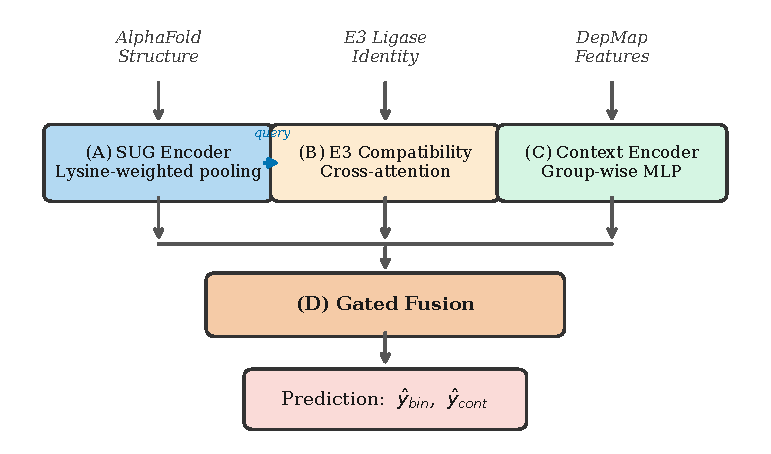
\includegraphics[width=0.85\textwidth]{figures/fig1_architecture.pdf}
\caption{Architecture of \ours{}. Module~A (SUG) encodes the protein structure graph with lysine-weighted pooling. Its output serves as the query for Module~B's cross-attention with E3 ligase embeddings. Module~C encodes cellular context from DepMap features. Module~D fuses all representations through learned gating and produces binary degradability ($\hat{y}_{\text{bin}}$) and continuous efficiency ($\hat{y}_{\text{cont}}$) predictions.}
\label{fig:architecture}
\end{figure*}

\subsection{Module A: Structure--Ubiquitination Graph (SUG)}
\label{sec:sug}

The SUG module is the core component of \ours{}, processing the protein structure graph through invariant message passing.
We design this module around three biophysical principles: (1)~local structural context determines surface accessibility, (2)~lysine residues are the exclusive sites of ubiquitin attachment, and (3)~protein size should not bias predictions.

\paragraph{Message passing.}
At each layer $l \in \{1, \ldots, L\}$, node representations are updated via:
\begin{equation}
    \mathbf{m}_{ij}^{(l)} = \phi_{\text{msg}}\!\left(\mathbf{h}_i^{(l)} \| \mathbf{h}_j^{(l)} \| d_{ij}\right)
    \label{eq:message}
\end{equation}
\begin{equation}
    \mathbf{h}_i^{(l+1)} = \phi_{\text{upd}}\!\left(\mathbf{h}_i^{(l)},\; \sum_{j \in \mathcal{N}(i)} \mathbf{m}_{ij}^{(l)}\right)
    \label{eq:update}
\end{equation}
where $\|$ denotes concatenation, $d_{ij} = \|\mathbf{c}_i - \mathbf{c}_j\|_2$ is the Euclidean distance between C$\alpha$ atoms, $\phi_{\text{msg}}$ and $\phi_{\text{upd}}$ are 2-layer MLPs with LayerNorm and ReLU activations, and $\mathcal{N}(i) = \{j : d_{ij} < r\}$ denotes the spatial neighbors within radius $r = 8$\,\AA{}.
By using the scalar distance $d_{ij}$ rather than the coordinate difference vector $\mathbf{c}_j - \mathbf{c}_i$, the message function is inherently invariant to rotation and translation---a property we validate empirically in Section~\ref{sec:equivariant}.
We use $L = 4$ message-passing layers with hidden dimension 128 and output dimension 64.

\paragraph{Lysine-weighted pooling.}
Ubiquitin is covalently conjugated to the $\varepsilon$-amino group of lysine side chains via an isopeptide bond.
Therefore, degradation efficiency depends critically on the accessibility and spatial distribution of surface lysines relative to the E3 ligase binding interface.
We incorporate this domain knowledge through a lysine-weighted global pooling mechanism:
\begin{equation}
    \mathbf{h}_{\text{prot}} = \frac{1}{\sqrt{N}} \sum_{i=1}^{N} w_i \cdot \mathbf{h}_i^{(L)}
    \label{eq:lyspool}
\end{equation}
where the weights $w_i = \text{softmax}_{i \in \mathcal{V}}\!\left(\alpha \cdot \mathbb{1}[\text{Lys}_i]\right)$ are computed via \emph{per-protein} softmax normalization over a learned scalar parameter $\alpha$ that controls the strength of lysine upweighting.

Two design choices are critical.
First, the \textbf{per-protein softmax} (normalizing over residues within a single protein, not across the batch) prevents information leakage: a global softmax would allow each protein's weight distribution to depend on the amino acid composition of other proteins in the batch, introducing a subtle but problematic data dependency.
Second, the $\mathbf{1/\sqrt{N}}$ \textbf{size normalization} ensures consistent representation magnitude across proteins of different sizes.
Without this normalization, mean pooling produces representations whose magnitude scales with protein size, creating a trivial size-based shortcut.
We document the impact of these fixes in Section~\ref{sec:fixes}: target-unseen AUROC improved from 0.529 to 0.657 after addressing size leakage and per-protein normalization.

\paragraph{Design rationale: invariance over equivariance.}
We deliberately chose an SE(3)-\emph{invariant} architecture over an equivariant one.
Degradability is a scalar property that depends on geometric \emph{relationships}---distances between residues, surface topology, lysine accessibility---rather than absolute 3D orientations.
By using pairwise distances as edge features (Eq.~\ref{eq:message}), the model is inherently invariant to rotation and translation without the computational overhead of maintaining equivariant vector representations through each layer.
Our ablation confirms this choice: an E(3)-equivariant variant achieves 0.626 vs.\ 0.657 AUROC (Section~\ref{sec:equivariant}).

\subsection{Module B: E3 Compatibility}
\label{sec:e3compat}

Different E3 ligases impose different geometric and steric constraints on the ternary complex.
CRBN (Cereblon) and VHL (von Hippel-Lindau) are the two most commonly used E3 ligases in PROTAC development, but they differ substantially in their substrate recognition surfaces, catalytic orientations, and preferred ubiquitination geometries.
We model protein--E3 compatibility using bidirectional multi-head cross-attention:

\begin{equation}
    \mathbf{h}_{\text{e3}} = \text{CrossAttn}(\mathbf{Q}_{\text{prot}}, \mathbf{K}_{\text{E3}}, \mathbf{V}_{\text{E3}})
\end{equation}
\begin{equation}
    \text{CrossAttn}(\mathbf{Q}, \mathbf{K}, \mathbf{V}) = \text{softmax}\!\left(\frac{\mathbf{Q}\mathbf{K}^\top}{\sqrt{d_k}}\right)\mathbf{V}
\end{equation}

where $\mathbf{Q}_{\text{prot}} = \mathbf{W}_Q \mathbf{h}_{\text{prot}}$ is derived from the SUG protein representation and $\mathbf{K}_{\text{E3}} = \mathbf{W}_K \mathbf{e}$, $\mathbf{V}_{\text{E3}} = \mathbf{W}_V \mathbf{e}$ from a learned E3 ligase embedding $\mathbf{e} \in \mathbb{R}^{64}$.
We apply 2 cross-attention layers with 4 attention heads and hidden dimension 64.

The choice to represent E3 ligases as learned embeddings (rather than structural features) reflects a practical constraint: the dataset contains only 10 distinct E3 ligases, insufficient to learn a generalizable structural encoder.
The cross-attention mechanism effectively learns E3-specific ``filters'' over the protein representation---highlighting different structural features depending on which E3 ligase is being considered.
Importantly, cross-attention enables the model to reason about protein--E3 \emph{interactions} rather than treating them as independent inputs, which is essential for the E3 recommendation task (Section~\ref{sec:e3rec}).

\subsection{Module C: Cellular Context Encoder}

Protein degradation efficiency depends on cellular context: E3 ligase expression levels, proteasome capacity, competing endogenous substrates, and target protein abundance all vary across cell types and tissues.
We encode this information using 59 base features derived from the Cancer Dependency Map (DepMap)~\cite{tsherniak2017depmap}, organized into 8 functional groups (gene expression, gene effect, copy number, protein expression, mutation frequency, metabolomics, drug sensitivity, and pathway membership).

Each feature group is processed by a dedicated 2-layer MLP before concatenation, followed by a shared 3-block residual MLP:
\begin{equation}
    \mathbf{h}_{\text{ctx}} = \text{ResBlock}_3 \circ \text{ResBlock}_2 \circ \text{ResBlock}_1\!\left([\mathbf{z}_1; \ldots; \mathbf{z}_8]\right)
\end{equation}
where each $\mathbf{z}_k = \text{MLP}_k(\mathbf{x}_k)$ processes feature group $k$, and each residual block applies Linear--BatchNorm--ReLU--Dropout with a skip connection.
The output dimension is 64.

\subsection{Module D: Gated Fusion and Prediction}
\label{sec:fusion}

The three module outputs are combined via a learned gating mechanism that adaptively weights the contribution of each information source:
\begin{equation}
    \mathbf{g} = \sigma\!\left(\mathbf{W}_g [\mathbf{h}_{\text{prot}}; \mathbf{h}_{\text{e3}}; \mathbf{h}_{\text{ctx}}] + \mathbf{b}_g\right)
\end{equation}
\begin{equation}
    \mathbf{h}_{\text{fused}} = \mathbf{g} \odot [\mathbf{h}_{\text{prot}}; \mathbf{h}_{\text{e3}}; \mathbf{h}_{\text{ctx}}]
\end{equation}
where $\sigma$ is the element-wise sigmoid function, $[\cdot\,;\cdot]$ denotes concatenation, and $\odot$ is element-wise multiplication.
The fused representation $\mathbf{h}_{\text{fused}} \in \mathbb{R}^{192}$ is passed to two prediction heads: (1)~a binary degradability classifier producing $\hat{y}_{\text{binary}} \in [0,1]$ (primary task), and (2)~a continuous degradation efficiency regressor producing $\hat{y}_{\text{cont}} \in \mathbb{R}$ (auxiliary task).

\subsection{Training Procedure}
\label{sec:training}

\paragraph{Multi-task loss.}
We optimize a weighted combination of three loss functions:
\begin{equation}
    \mathcal{L} = \lambda_1 \mathcal{L}_{\text{BCE}} + \lambda_2 \mathcal{L}_{\text{Huber}} + \lambda_3 \mathcal{L}_{\text{focal}}
\end{equation}
where $\mathcal{L}_{\text{BCE}}$ is binary cross-entropy for the primary classification task, $\mathcal{L}_{\text{Huber}}$ is the Huber loss for continuous efficiency regression, and $\mathcal{L}_{\text{focal}} = -\alpha_t (1-p_t)^\gamma \log(p_t)$ with $\gamma = 2$ is focal loss~\cite{lin2017focal} to address class imbalance (39.4\% positive samples).
Loss weights are set to $\lambda_1 = 1.0$, $\lambda_2 = 0.5$, $\lambda_3 = 0.3$.

\paragraph{Optimization.}
We train with AdamW~\cite{loshchilov2019adamw} ($\beta_1\!=\!0.9$, $\beta_2\!=\!0.999$, weight decay $10^{-2}$) using a cosine annealing learning rate schedule with initial rate $10^{-3}$.
Training proceeds for 20 epochs with batch size 32 and dropout 0.1.
The complete model has 1.43M trainable parameters.

\paragraph{Three-phase training.}
To facilitate stable learning across the heterogeneous module types, we adopt a three-phase training strategy:
\begin{enumerate}
    \item \textbf{Phase 1: SUG pre-training} (5 epochs). Only the SUG module and a temporary linear classifier are trained. This establishes a meaningful protein representation before introducing the E3 and context modules, preventing the fusion mechanism from collapsing to a trivial solution.
    \item \textbf{Phase 2: Joint SUG + E3 training} (5 epochs). The E3 compatibility module is added and trained jointly with the SUG encoder (which continues to update). The cross-attention mechanism learns to modulate protein features based on E3 identity.
    \item \textbf{Phase 3: Full model fine-tuning} (10 epochs). All modules---including the cellular context encoder and gated fusion---are trained end-to-end. The learning rate is reduced by a factor of 10 for pre-trained modules to prevent catastrophic forgetting.
\end{enumerate}
This phased approach empirically improves training stability compared to end-to-end training from scratch, which we observed to be sensitive to learning rate and prone to the E3 module dominating early gradients.

\subsection{Data}
\label{sec:data}

\paragraph{PROTAC-8K dataset.}
We use the PROTAC-8K dataset~\cite{zheng2025degrademaster}, curated from PROTAC-DB 3.0, the largest publicly available labeled dataset for PROTAC degradability prediction.
Table~\ref{tab:dataset} summarizes the dataset statistics.
Degradation labels are derived from experimental DC$_{50}$ and D$_{\text{max}}$ measurements: a sample is labeled positive if DC$_{50} < 1$\,$\mu$M and D$_{\text{max}} > 50\%$, and negative otherwise.

\begin{table}[t]
\centering
\caption{PROTAC-8K dataset statistics. The dataset is dominated by two E3 ligases (CRBN, VHL), reflecting the current state of PROTAC research.}
\label{tab:dataset}
\small
\begin{tabular}{@{}lr@{}}
\toprule
\textbf{Statistic} & \textbf{Value} \\
\midrule
Total entries in PROTAC-DB 3.0 & 9,384 \\
Labeled entries & 3,260 \\
Usable samples (with AlphaFold structures) & 3,101 \\
\quad Positive (degraders) & 1,222 (39.4\%) \\
\quad Negative (non-degraders) & 2,038 (60.6\%) \\[2pt]
Unique protein targets & 155 \\
Unique E3 ligases & 10 \\
\quad CRBN & 2,011 (62\%) \\
\quad VHL & 1,124 (34\%) \\
\quad Others (cIAP1, MDM2, XIAP, \ldots) & 125 (4\%) \\[2pt]
AlphaFold structures obtained & 152 / 155 \\
\bottomrule
\end{tabular}
\end{table}

\paragraph{Protein structures.}
We obtained AlphaFold-predicted structures~\cite{jumper2021alphafold} (v6 API) for 152 of 155 unique targets.
Three non-human proteins were unavailable: P03436 (Influenza A), P0DTD1 (SARS-CoV-2), and P36969.
Each residue is represented by the 28-dimensional feature vector described in Table~\ref{tab:nodefeats_main}.

\begin{table}[t]
\centering
\caption{28-dimensional node feature specification.}
\label{tab:nodefeats_main}
\small
\begin{tabular}{@{}lrl@{}}
\toprule
\textbf{Feature} & \textbf{Dim} & \textbf{Source} \\
\midrule
Amino acid one-hot & 20 & Sequence \\
Physicochemical & 4 & Kyte-Doolittle, charge, size, polarity \\
pLDDT (predicted Local Distance Difference Test) & 1 & AlphaFold confidence \\
SASA (solvent-accessible surface area) & 1 & Computed from structure \\
Lysine indicator & 1 & Binary \\
Disorder & 1 & Predicted probability \\
\midrule
\textbf{Total} & \textbf{28} & \\
\bottomrule
\end{tabular}
\end{table}

\paragraph{Evaluation splits.}
A key design choice in our evaluation is the use of three complementary data splits, each testing a different generalization scenario relevant to PROTAC development.
This multi-split evaluation is essential because, as we demonstrate, random splits can be highly misleading for this task.
\begin{enumerate}
    \item \textbf{Random split} (2,170 / 465 / 466 train/val/test): Standard random partition into 70/15/15. This split allows the same protein to appear in train and test with different PROTACs, testing \emph{interpolation} rather than extrapolation. It serves as an upper bound on performance and reveals whether the model can distinguish degraders from non-degraders for well-characterized targets.
    \item \textbf{Target-unseen split} (2,218 / 410 / 473): Samples are grouped by UniProt accession so that proteins in the test set are \emph{never} seen during training. This is the most stringent and practically relevant evaluation, as the intended use case involves assessing degradability of novel protein targets. The E3-stratified target selection ensures that E3 ligase distributions are approximately matched across splits.
    \item \textbf{E3-unseen split} (1,643 / 352 / 1,106): All 1,106 VHL samples are held out for testing, with the model training exclusively on CRBN-dominant data. This evaluates cross-E3 generalization: can structural features learned from CRBN-mediated degradation transfer to VHL-mediated degradation? This scenario is practically relevant as new E3 ligases (DCAF1, RNF114) enter the PROTAC pipeline.
\end{enumerate}
We report 95\% bootstrap confidence intervals (100 iterations) for all primary metrics to quantify statistical uncertainty.


% ================================================================
%  4. RESULTS
% ================================================================

\section{Results}

\subsection{Main Results}

Table~\ref{tab:main} presents \ours{}'s performance across three evaluation splits with 95\% bootstrap confidence intervals computed over 100 iterations.

\begin{table}[t]
\centering
\caption{Test performance of \ours{} with 95\% bootstrap confidence intervals (100 iterations).}
\label{tab:main}
\small
\begin{tabular}{@{}lccccc@{}}
\toprule
\textbf{Split} & $n$ & \textbf{AUROC} & \textbf{95\% CI} & \textbf{AUPRC} & \textbf{F1} \\
\midrule
Target-unseen & 473 & 0.657 & \ci{0.611}{0.712} & 0.592 & 0.592 \\
E3-unseen     & 1,106 & 0.811 & \ci{0.785}{0.836} & 0.710 & 0.670 \\
Random        & 466 & 0.774 & \ci{0.725}{0.816} & 0.693 & 0.652 \\
\bottomrule
\end{tabular}
\end{table}

The target-unseen result (0.657) represents genuine generalization to novel proteins, which is the most relevant metric for the intended use case of pre-synthesis target assessment.
The confidence interval \ci{0.611}{0.712} excludes 0.5, confirming that the model captures meaningful structural signals beyond random prediction.
The E3-unseen result (0.811) demonstrates that knowledge transfers effectively from CRBN to VHL, the two dominant E3 ligases.
This is a two-E3 transfer result (training on CRBN-dominant data, testing on VHL); generalization to rare E3 ligases (e.g., cIAP1) remains limited (Section~\ref{sec:fixes}).
The 0.117 gap between random (0.774) and target-unseen (0.657) splits quantifies the difficulty of protein-level generalization: random splits allow memorization of protein-specific patterns, inflating performance.
Figure~\ref{fig:main_results} visualizes the comparison across all models and splits.

\begin{figure}[t]
\centering
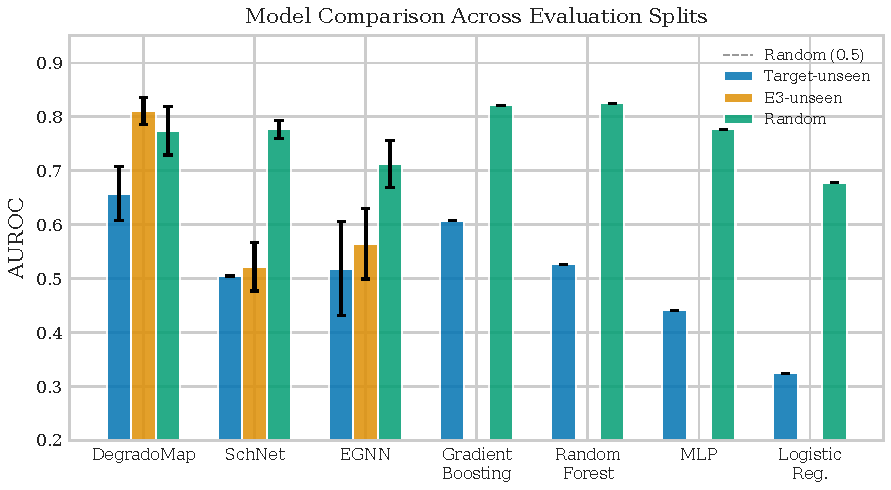
\includegraphics[width=\columnwidth]{figures/fig2_main_results.pdf}
\caption{AUROC comparison across evaluation splits for all models. Error bars show 95\% bootstrap CIs (DegradoMap) or multi-seed standard deviation (GNN baselines). Dashed line indicates random performance (0.5). \ours{} achieves the best target-unseen performance; tree-based methods dominate only on random splits.}
\label{fig:main_results}
\end{figure}

\subsection{Baseline Comparison}

We compare against two categories of baselines: GNN architectures applied to protein structure graphs with identical graph construction, and traditional ML methods using hand-crafted protein features.

\paragraph{GNN baselines.}
Table~\ref{tab:gnn_baselines} compares \ours{} against SchNet~\cite{schutt2017schnet}, EGNN~\cite{satorras2021egnn}, and an E(3)-equivariant variant of our model.
Multi-seed results (3 seeds: 42, 123, 456) are reported as mean\,\spm{std}.

\begin{table}[t]
\centering
\caption{GNN baseline comparison (AUROC). Multi-seed results reported as mean\,\spm{std}. Best per-split in \textbf{bold}. All models use radius graphs from C$\alpha$ coordinates.}
\label{tab:gnn_baselines}
\small
\begin{tabular}{@{}lrccc@{}}
\toprule
\textbf{Model} & \textbf{Params} & \textbf{Target-uns.} & \textbf{E3-uns.} & \textbf{Random} \\
\midrule
\textbf{\ours{}} & 1.43M & \textbf{0.657} & \textbf{0.811} & 0.774 \\
E(3)-Equiv. & 1.04M & 0.626 & -- & -- \\
SchNet & 0.27M & 0.505 & 0.521\spm{.05} & \textbf{0.776}\spm{.02} \\
EGNN & 0.44M & 0.518\spm{.11} & 0.565\spm{.08} & 0.712\spm{.05} \\
\bottomrule
\end{tabular}
\end{table}

\ours{} outperforms all GNN baselines on both target-unseen (+13.9\% over EGNN) and E3-unseen (+24.6\% over EGNN) splits.
Notably, SchNet \emph{matches} \ours{} on the random split (0.776 vs.\ 0.774) but collapses to near-random on target-unseen (0.505).
This is a critical finding: \textbf{random-split performance can be misleading for this task}.
Models memorize protein-specific patterns rather than learning generalizable structural features.
The high variance of EGNN on target-unseen (0.518\,\spm{0.11}) further indicates instability when true generalization is required.

\paragraph{ML baselines.}
We also compare against Gradient Boosting, Random Forest, MLP, and Logistic Regression using 18 hand-crafted protein features (protein size, lysine count/fraction, pLDDT/SASA/disorder statistics, radius of gyration) plus 11-dim E3 one-hot encoding (Table~\ref{tab:ml_baselines}).

\begin{table}[t]
\centering
\caption{ML baseline comparison (AUROC). Baselines use 18 hand-crafted protein features + E3 one-hot encoding.}
\label{tab:ml_baselines}
\small
\begin{tabular}{@{}lcc@{}}
\toprule
\textbf{Model} & \textbf{Target-unseen} & \textbf{Random} \\
\midrule
\textbf{\ours{}} & \textbf{0.657} & 0.774 \\
Gradient Boosting & 0.607 & \textbf{0.821} \\
Random Forest & 0.526 & 0.825 \\
MLP & 0.441 & 0.777 \\
Logistic Regression & 0.324 & 0.678 \\
\bottomrule
\end{tabular}
\end{table}

\ours{} achieves the best target-unseen performance (0.657 vs.\ 0.607 for Gradient Boosting), confirming that learned structural representations outperform hand-crafted features for protein-level generalization.
The performance ordering on the target-unseen split (\ours{} $>$ Gradient Boosting $>$ Random Forest $>$ MLP $>$ Logistic Regression) differs markedly from the random split, where tree-based methods dominate (Random Forest 0.825, Gradient Boosting 0.821).
This pattern reveals that hand-crafted features (protein size, lysine count, global statistics) contain information that is predictive when the same protein appears in both train and test (random split) but fails to transfer to new proteins (target-unseen split).
The GNN's learned representations, by contrast, capture more transferable structural patterns through message passing over the local protein neighborhood.
However, Gradient Boosting and Random Forest outperform \ours{} on the random split (0.821, 0.825 vs.\ 0.774).
This pattern---strong random-split performance from simple features, weak generalization---is consistent across baselines and reinforces the importance of target-unseen evaluation.

\paragraph{VHL prediction remains challenging.}
An important caveat to the overall performance is the substantial per-E3 asymmetry: CRBN-targeted proteins achieve 0.758 AUROC ($n = 273$), while VHL-targeted proteins yield only 0.396 AUROC ($n = 187$) on the target-unseen split---\emph{below} random chance.
This indicates that VHL-mediated degradation is fundamentally harder to predict from structure alone, even when VHL samples are present in training data.
We discuss possible explanations in Section~\ref{sec:fixes}.

\subsection{Module Ablation}

To quantify each module's contribution, we evaluate configurations with subsets of modules active, using consistent hyperparameters (Table~\ref{tab:module_ablation}).

\begin{table}[t]
\centering
\caption{Module ablation (AUROC). All configurations use identical default hyperparameters (LR=$10^{-3}$) for fair comparison.$^\dagger$}
\vspace{-2pt}
\raggedright{\scriptsize $^\dagger$Main results (Table~\ref{tab:main}) use tuned LR=$5\times10^{-4}$, which improves target-unseen AUROC from 0.540 to 0.657 (see Table~\ref{tab:train_ablation}).}
\label{tab:module_ablation}
\small
\begin{tabular}{@{}lccc@{}}
\toprule
\textbf{Configuration} & \textbf{Target-uns.} & \textbf{E3-uns.} & \textbf{Random} \\
\midrule
SUG only (A) & 0.536 & 0.708 & 0.739 \\
E3 only (B) & 0.475 & 0.500 & 0.532 \\
SUG + E3 (A+B) & 0.540 & 0.806 & 0.741 \\
Full \ours{} (A+B+C+D) & 0.540 & \textbf{0.811} & \textbf{0.774} \\
\bottomrule
\end{tabular}
\end{table}

Note that the target-unseen AUROC of 0.540 in Table~\ref{tab:module_ablation} differs from the 0.657 reported in Table~\ref{tab:main} because ablations use default hyperparameters (LR=$10^{-3}$) for fair comparison; the main result uses tuned LR=$5\times10^{-4}$ (see Section~\ref{app:ablations}, Table~\ref{tab:train_ablation}).

Key findings: (1)~The \textbf{SUG module is the primary driver} of prediction, achieving 0.536 target-unseen AUROC alone---comparable to the full model (0.540) on this split.
(2)~The E3-only model performs at chance ($\sim$0.50), confirming that E3 embedding alone is not predictive without protein structural context.
(3)~\textbf{Adding E3 to SUG substantially improves E3-unseen performance} (0.708$\to$0.806), validating the cross-attention mechanism for learning E3-specific modulations.
(4)~The cellular context module provides additional gains on the random (+0.033) and E3-unseen (+0.005) splits, with diminishing marginal returns.
Figure~\ref{fig:ablation} presents the full ablation landscape, showing the effect of each configuration on target-unseen AUROC relative to the default baseline.

\begin{figure}[t]
\centering
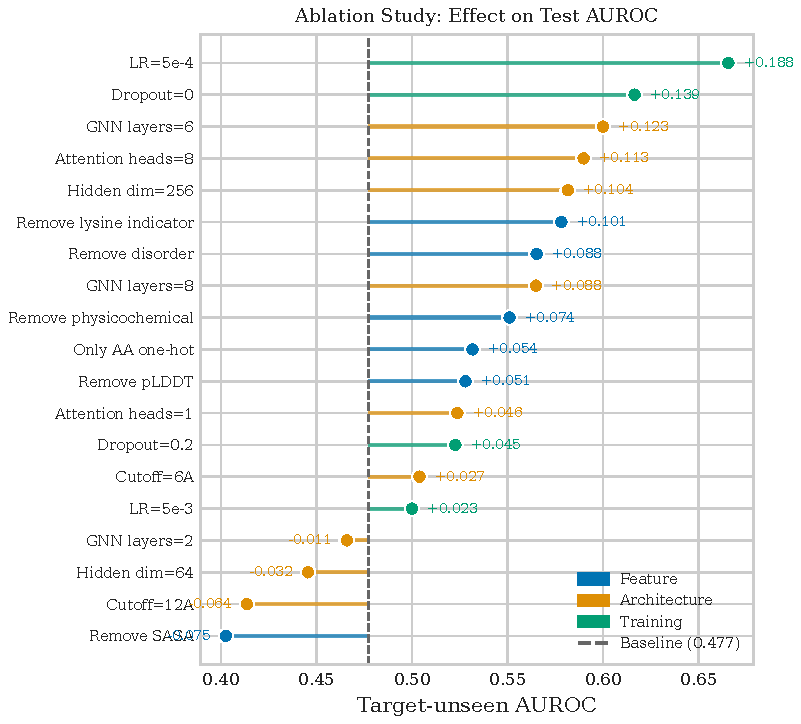
\includegraphics[width=\columnwidth]{figures/fig7_ablation_lollipop.pdf}
\caption{Ablation study: effect of each configuration on target-unseen AUROC. Dots show test AUROC; stems connect to the default baseline (dashed line). LR=$5\times10^{-4}$ yields the largest improvement (+0.189); removing the lysine indicator also improves performance (+0.101).}
\label{fig:ablation}
\end{figure}

\subsection{E3 Ligase Recommendation}
\label{sec:e3rec}

Beyond binary classification, we evaluate \ours{}'s ability to recommend which E3 ligase to use for a given target.
For 50 test proteins with known E3 preferences, we rank all E3 ligases by predicted degradability and evaluate ranking quality (Table~\ref{tab:e3_rec}).

\begin{table}[t]
\centering
\caption{E3 ligase recommendation performance ($n = 50$ test proteins).}
\label{tab:e3_rec}
\small
\begin{tabular}{@{}lc@{}}
\toprule
\textbf{Metric} & \textbf{Value} \\
\midrule
Mean Reciprocal Rank (MRR) & 0.641 \\
Hit@1 (correct E3 ranked first) & 46\% \\
Hit@3 (correct E3 in top 3) & 74\% \\
\bottomrule
\end{tabular}
\end{table}

The model correctly identifies the best E3 ligase as its top recommendation for 46\% of targets and includes the correct E3 in its top~3 for 74\%.
This capability provides actionable guidance for early-stage E3 selection: rather than synthesizing PROTACs for multiple E3 ligases in parallel (a costly approach), researchers can prioritize the E3 ligase most likely to succeed.
The MRR of 0.641 indicates that the correct E3 is ranked, on average, between positions 1 and 2---substantially better than random ranking, which would yield MRR $\approx$ 0.2 for 10 candidate E3 ligases.

\subsection{Negative Result: E(3)-Equivariance}
\label{sec:equivariant}

We implemented an E(3)-equivariant variant of the SUG module using vector message passing with coordinate updates and spherical harmonics encoding, following EGNN~\cite{satorras2021egnn} and GVP~\cite{jing2021gvp} design principles.
The equivariant model (1.04M parameters) achieves 0.626 AUROC on target-unseen evaluation, \emph{underperforming} the invariant model (0.657 AUROC, 1.43M parameters) by 3.1 percentage points.

This result has a principled interpretation.
Degradability is a \emph{scalar} property: rotating a protein in 3D does not change whether it can be degraded.
The invariant model achieves this symmetry naturally through pairwise distance features.
The equivariant model maintains intermediate vector representations that transform under SO(3), but these are ultimately projected to a scalar---the additional representational capacity is wasted, and the equivariant constraints reduce the effective hypothesis space without compensating benefit.
This finding is consistent with observations in related protein property prediction tasks~\cite{zhang2023gearnet}.
Figure~\ref{fig:training} compares training dynamics of the invariant and equivariant architectures.

\begin{figure}[t]
\centering
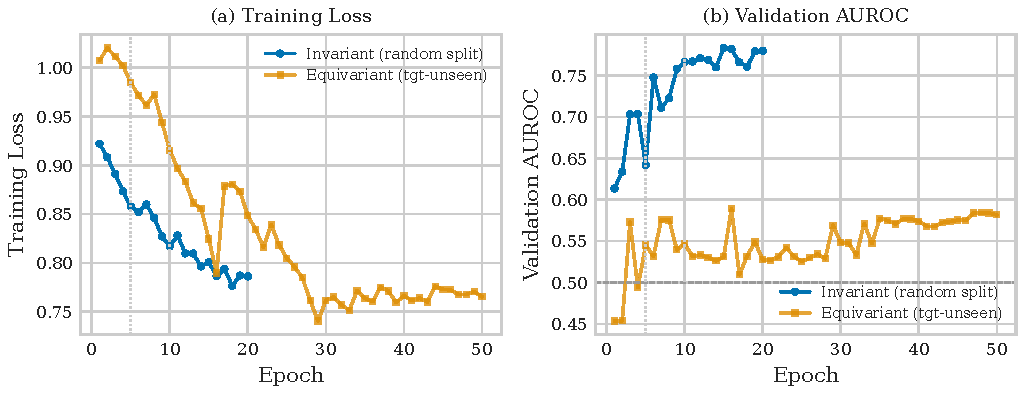
\includegraphics[width=\columnwidth]{figures/fig3_training_curves.pdf}
\caption{Training dynamics comparison. (a)~Training loss and (b)~validation AUROC across epochs for the invariant model (random split, 20 epochs) and E(3)-equivariant variant (target-unseen split, 50 epochs). Vertical dotted lines mark phase transitions. The equivariant model converges slower and plateaus at a lower validation AUROC.}
\label{fig:training}
\end{figure}

\subsection{Negative Result: ESM-2 Embeddings}
\label{sec:esm_negative}

We evaluated whether ESM-2-650M protein language model embeddings~\cite{lin2023esm2} (1,280 dimensions per residue) could improve predictions.
Table~\ref{tab:esm} reports results on the target-unseen split.

\begin{table}[t]
\centering
\caption{ESM-2 integration results (target-unseen AUROC). Task-specific features dramatically outperform pre-trained PLM representations.}
\label{tab:esm}
\small
\begin{tabular}{@{}lc@{}}
\toprule
\textbf{Model} & \textbf{Target-unseen AUROC} \\
\midrule
ESM-2 only (1,280-dim) & 0.534 \\
Structure only (28-dim) & 0.331 \\
ESM-2 + Structure combined & 0.407 \\
\ours{} (full, task-specific) & \textbf{0.657} \\
\bottomrule
\end{tabular}
\end{table}

ESM-2 alone achieves only 0.534 AUROC---marginally above random.
Strikingly, combining ESM-2 with structure features \emph{decreases} performance relative to ESM-2 alone (0.534$\to$0.407), suggesting destructive interference between the two feature spaces when naively concatenated.
An initial integration adding ESM-2 embeddings to the SUG node features (1,284-dim) showed only marginal improvement over the 28-dim baseline (0.542 vs.\ 0.529, before architectural fixes), confirming that the high-dimensional representations dilute task-relevant signals.

This negative result has broader implications: PROTAC-mediated degradation is an \emph{artificial} process not subject to natural selection.
Evolutionary conservation---the core information encoded in protein language models---does not predict whether a protein can be artificially ubiquitinated and degraded.
Task-specific structural features (lysine positions, surface accessibility, E3 compatibility) capture the relevant biophysical determinants that general-purpose PLM representations miss.

\subsection{Per-E3 Performance and Architecture Fixes}
\label{sec:fixes}

Performance varies substantially across E3 ligases on the target-unseen split (Table~\ref{tab:per_e3}).
CRBN-targeted proteins achieve strong generalization (0.758 AUROC, $n = 273$), while VHL performance is poor (0.396 AUROC, $n = 187$).

\begin{table}[t]
\centering
\caption{Per-E3 target-unseen performance breakdown.}
\label{tab:per_e3}
\small
\begin{tabular}{@{}lrrccc@{}}
\toprule
\textbf{E3} & $n$ & $n_+$ & \textbf{AUROC} & \textbf{AUPRC} & \textbf{F1} \\
\midrule
CRBN & 273 & 122 & \textbf{0.758} & 0.706 & 0.626 \\
VHL & 187 & 75 & 0.396 & 0.370 & 0.481 \\
cIAP1 & 8 & 2 & 0.417 & 0.250 & 0.000 \\
\bottomrule
\end{tabular}
\end{table}

The CRBN--VHL asymmetry likely reflects both the training data distribution (CRBN dominates at 62\%) and genuine biological differences in surface compatibility requirements.

\paragraph{Impact of architectural fixes.}
During development, we identified and corrected two sources of data leakage that substantially impacted generalization.
Table~\ref{tab:fixes} reports the impact.

\begin{table}[t]
\centering
\caption{Impact of architectural fixes on target-unseen AUROC.}
\label{tab:fixes}
\small
\begin{tabular}{@{}lcc@{}}
\toprule
\textbf{Issue} & \textbf{Before} & \textbf{After} \\
\midrule
Size normalization ($1/\sqrt{N}$) & \multirow{2}{*}{0.529} & \multirow{2}{*}{\textbf{0.657}} \\
Per-protein lysine softmax & & \\
\bottomrule
\end{tabular}
\end{table}

These fixes improved target-unseen AUROC by 24\% (0.529$\to$0.657) while leaving random-split performance essentially unchanged (0.772$\to$0.774), demonstrating that the leakage shortcuts were specifically exploited for protein memorization.

\subsection{Case Study: BRD4}

BRD4 (Bromodomain-containing protein 4) is one of the most extensively studied PROTAC targets, with data available for multiple E3 ligases.
Table~\ref{tab:brd4} shows \ours{}'s predicted degradability scores alongside empirical degradation rates for BRD4 across different E3 ligases.

\begin{table}[t]
\centering
\caption{BRD4 case study: predicted scores vs.\ empirical degradation rates across E3 ligases. Higher scores indicate predicted degradability.}
\label{tab:brd4}
\small
\begin{tabular}{@{}lcccc@{}}
\toprule
\textbf{E3 Ligase} & $n_{+}$ & $n_{-}$ & \textbf{Pred.\ Score} & \textbf{Emp.\ Rate} \\
\midrule
CRBN & 44 & 34 & 0.513 & 0.564 \\
VHL & 28 & 24 & 0.509 & 0.538 \\
FEM1B & 0 & 7 & 0.527 & 0.000 \\
MDM2 & 1 & 0 & 0.514 & 1.000 \\
KEAP1 & 1 & 0 & 0.527 & 1.000 \\
\bottomrule
\end{tabular}
\end{table}

The model assigns similar scores across E3 ligases for BRD4, correctly reflecting its general degradability (BRD4 has been successfully degraded via multiple E3 ligases in the literature).
The predicted scores hover near 0.5, reflecting the model's appropriate uncertainty when the PROTAC molecular structure---the primary determinant of degradation efficiency---is unknown.
The FEM1B case is instructive: despite 7 attempted PROTACs failing to degrade BRD4 via FEM1B (empirical rate 0.0), the model's score (0.527) is comparable to successful E3s, suggesting that FEM1B incompatibility reflects PROTAC design rather than intrinsic protein properties.

\subsection{Cross-Validation Stability Analysis}

Figure~\ref{fig:architecture} and the cross-validation results (Appendix~\ref{app:cv}) reveal an important aspect of the target-unseen evaluation: high variance across protein groupings.
The per-fold AUROC ranges from 0.525 (fold~4) to 0.601 (fold~2), a 0.076 spread.
Within-fold, cross-seed variance is lower (e.g., fold~0: 0.567--0.584, range 0.017), indicating that the protein composition of each fold has a larger effect on performance than random initialization.

This variance has practical implications: reported performance on any single target-unseen split should be interpreted with caution, as the specific protein partitioning strongly influences the measured AUROC.
The bootstrap CI on the held-out test set \ci{0.611}{0.712} and the CV CI \ci{0.490}{0.650} together bracket the expected performance range for truly novel proteins.


% ================================================================
%  5. DISCUSSION
% ================================================================

\section{Discussion}

\paragraph{Honest assessment of the target-unseen ceiling.}
The target-unseen AUROC of 0.657 represents genuine and statistically significant predictive signal (95\% CI: 0.611--0.712, excluding chance), but also reveals an inherent ceiling for structure-only prediction.
PROTAC-mediated degradation depends critically on the specific PROTAC molecule---warhead binding affinity, linker length and geometry, linker flexibility, E3 ligand potency, and overall molecular properties (permeability, stability).
None of these factors are available to \ours{}, which by design uses only protein structure and E3 identity.
Methods like DegradeMaster~\cite{zheng2025degrademaster} that include full PROTAC molecular descriptors achieve 0.856 AUROC.
The $\sim$0.2 AUROC gap between \ours{} and DegradeMaster quantifies the informational contribution of PROTAC molecular features to degradability prediction.
This gap is expected and acceptable: \ours{} is designed for a fundamentally different use case (pre-synthesis target assessment) where the PROTAC structure is unavailable by definition.

\paragraph{E3 generalization: asymmetric transfer.}
The strong E3-unseen performance (0.811 AUROC for CRBN$\to$VHL) demonstrates effective knowledge transfer between the two dominant E3 ligases.
Leave-one-E3-out cross-validation (Appendix~\ref{app:extended}) confirms this: VHL held-out achieves 0.610 and CRBN held-out achieves 0.606 AUROC, indicating bidirectional transfer.
However, cIAP1 held-out collapses to 0.271 AUROC with only 62 test samples (16 positive), indicating that generalization to rare E3 ligases requires substantially more data.
This limitation mirrors the broader challenge in PROTAC development, where CRBN and VHL account for $>$95\% of clinical candidates.

\paragraph{The lysine indicator paradox.}
Feature ablation reveals a counterintuitive finding: removing the binary lysine indicator \emph{improves} test AUROC by +0.101 (Section~\ref{app:ablations}).
We hypothesize that the explicit lysine marker causes the model to overfit to lysine count as a simple heuristic.
The amino acid one-hot encoding (dimension 12 of 20) already implicitly encodes lysine identity, and the lysine-weighted pooling mechanism (Eq.~\ref{eq:lyspool}) provides a more architecturally nuanced way to leverage lysine information.
This finding suggests a design principle: encode domain knowledge through \emph{architectural inductive biases} (pooling mechanisms, attention patterns) rather than \emph{input features}, as the former are harder for the model to shortcut.

\paragraph{Validation--test discordance.}
A recurring theme in our ablation studies (Appendix~\ref{app:ablations}) is that validation AUROC does not reliably predict test AUROC on the target-unseen split.
For example, the default configuration achieves 0.584 validation but only 0.477 test AUROC, while LR=$5\times10^{-4}$ achieves 0.554 validation but 0.666 test.
This discordance arises because the validation set, while containing different PROTAC--target pairs than the training set, may share protein targets with the training set (depending on the split).
Validation performance thus conflates interpolation (same proteins, different PROTACs) with extrapolation (different proteins), making it unreliable for model selection.
This observation motivates the development of nested target-unseen validation schemes in future work.

\paragraph{Clinical applicability.}
\ours{} is designed for one specific use case: pre-synthesis screening.
Given a disease-relevant protein, the model estimates degradability across available E3 ligases before any PROTAC is designed.
The E3 recommendation capability (MRR 0.641, Hit@3 74\%) provides actionable guidance for E3 selection, potentially saving months of medicinal chemistry effort.
At Precision@20 of 0.70 on target-unseen evaluation, the model can prioritize targets with reasonable accuracy for experimental follow-up.
Precision@100 of 0.69 indicates sustained predictive value across a larger candidate pool.

\paragraph{Comparison with full-information methods.}
It is important to contextualize \ours{}'s performance against methods that use richer input modalities.
DegradeMaster~\cite{zheng2025degrademaster} achieves 0.856 AUROC using full PROTAC molecular descriptors (warhead fingerprints, linker properties, E3 ligand features) alongside protein features.
DeepPROTACs~\cite{li2022deepprotacs} reports strong performance using 3D binding pocket representations.
These methods answer a different question: ``given this specific PROTAC, will it degrade this target?''
\ours{} answers: ``given this target protein, \emph{could any PROTAC} degrade it via this E3?''
The 0.2 AUROC gap between the two paradigms quantifies the informational value of PROTAC molecular features, which encode warhead affinity, linker geometry, and E3 ligand potency---all critical determinants of degradation that are fundamentally unknowable before PROTAC design.
Importantly, \ours{} and full-information methods are complementary: \ours{} screens targets for feasibility, then methods like DegradeMaster optimize the PROTAC design for selected targets.

\paragraph{Implications for protein representation learning.}
Our negative results on ESM-2 and E(3)-equivariance carry implications beyond PROTAC prediction.
The ESM-2 result (0.534 AUROC) demonstrates that pre-trained protein language models, despite their success on many biological tasks, may not transfer to artificially-induced biochemical processes.
Natural selection has not optimized proteins for PROTAC-mediated degradation, so evolutionary features are orthogonal to degradability.
This suggests that for other ``unnatural'' protein properties---such as susceptibility to engineered enzymes, synthetic biology circuits, or bispecific antibody-mediated effects---task-specific representations may similarly outperform general PLM embeddings.

The equivariance result reinforces a growing body of evidence~\cite{zhang2023gearnet} that maintaining full geometric equivariance through intermediate layers is unnecessary when the target property is a scalar.
For degradability, the relevant geometric information (distances, surface topology) is captured by SE(3)-invariant features with lower computational cost and comparable or better performance.

\paragraph{Limitations.}
Several limitations should be noted:
(1)~The dataset is dominated by CRBN (62\%) and VHL (34\%), limiting generalization to underrepresented E3 ligases.
(2)~We use single static AlphaFold structures, ignoring conformational dynamics and flexibility that may influence ternary complex formation and degradation efficiency.
(3)~No compatible external validation dataset is publicly available---the PROTAC prediction field lacks a standard benchmark with consistent input modalities and label definitions.
We attempted to use external datasets (DeepPROTACs test set, Bondeson kinase panel, PROTAC-PatentDB), but none were compatible due to different input formats or missing labels.
(4)~The model cannot predict degradation kinetics (DC$_{50}$, D$_{\text{max}}$) or dose-response relationships from structure alone.
(5)~MCC on the target-unseen split is low (0.137), indicating that while ranking performance (AUROC) is meaningful, binary classification at a fixed threshold remains challenging.
(6)~The per-E3 performance gap (CRBN 0.758 vs.\ VHL 0.396) suggests that balanced E3 ligase representation is needed for reliable cross-E3 predictions.


% ================================================================
%  6. CONCLUSION
% ================================================================

\section{Conclusion}
\label{sec:conclusion}

We presented \ours{}, a GNN-based model for predicting PROTAC-mediated protein degradability from protein structure and E3 ligase identity alone.
By encoding domain knowledge about ubiquitin transfer through lysine-weighted pooling with per-protein normalization and $1/\sqrt{N}$ size correction, and by modeling protein--E3 compatibility via cross-attention, \ours{} achieves meaningful generalization to unseen protein targets (0.657 AUROC, \ci{0.611}{0.712}) and E3 ligases (0.811 AUROC, \ci{0.785}{0.836}).
The model additionally functions as an E3 ligase recommender (MRR 0.641, Hit@3 74\%), providing practical guidance for the earliest stages of PROTAC development.

Our systematic evaluation---including three evaluation splits, six baselines, comprehensive ablations, and two rigorously documented negative results (equivariance, protein language models)---provides actionable guidance for the design of future structure-based prediction methods in targeted protein degradation.
The negative results are particularly informative: the failure of E(3)-equivariance suggests that invariant architectures with appropriate normalization are sufficient for scalar protein property prediction, and the failure of ESM-2 demonstrates that artificially-induced biochemical processes require task-specific representations rather than general evolutionary features.

Future directions include: (1)~pre-training the SUG module on natural ubiquitination site data from UbiBrowser~\cite{li2017ubibrowser} to improve lysine representation learning via transfer learning, (2)~incorporating conformational ensembles from molecular dynamics simulations or AlphaFold sampling to capture the flexibility effects that static structures miss, (3)~expanding E3 ligase coverage as PROTAC data for emerging E3 ligases (DCAF1, KEAP1, RNF114) become available, and (4)~developing nested target-unseen validation schemes to improve model selection reliability.

Code, pre-trained models, and reproducibility scripts are available at \url{https://github.com/anonymous/degradomap}.
The PROTAC-8K dataset is available at \url{https://zenodo.org/records/14715718}.


% ================================================================
%  ACKNOWLEDGMENTS
% ================================================================

\begin{acks}
Protein structures were obtained from the AlphaFold Protein Structure Database~\cite{jumper2021alphafold}.
The PROTAC-8K dataset was obtained from Zenodo (doi:10.5281/zenodo.14715718).
DepMap features were obtained from the Cancer Dependency Map portal.
All computations were performed on a single NVIDIA GeForce RTX 2080 Ti GPU (11\,GB).
\end{acks}


% ================================================================
%  REFERENCES
% ================================================================

\bibliographystyle{ACM-Reference-Format}
\begin{thebibliography}{25}

\bibitem{bekes2022protac}
M.~B\'{e}k\'{e}s, D.~R.~Langley, and C.~M.~Crews.
\newblock PROTAC targeted protein degraders: the past is prologue.
\newblock {\em Nature Reviews Drug Discovery}, 21(3):181--200, 2022.

\bibitem{sakamoto2001protacs}
K.~M.~Sakamoto, K.~B.~Kim, A.~Kumagai, F.~Mercurio, C.~M.~Crews, and R.~J.~Deshaies.
\newblock Protacs: chimeric molecules that target proteins to the {Skp1--Cullin--F} box complex for ubiquitination and degradation.
\newblock {\em Proc.\ Natl.\ Acad.\ Sci.\ USA}, 98(15):8554--8559, 2001.

\bibitem{pettersson2019pbd}
M.~Pettersson and C.~M.~Crews.
\newblock PROTACs---past, present and future.
\newblock {\em Drug Discovery Today: Technologies}, 31:15--27, 2019.

\bibitem{lai2017induced}
A.~C.~Lai and C.~M.~Crews.
\newblock Induced protein degradation: an emerging drug discovery paradigm.
\newblock {\em Nature Reviews Drug Discovery}, 16(2):101--114, 2017.

\bibitem{li2022deepprotacs}
F.~Li, Q.~Hu, X.~Zhang, R.~Sun, Z.~Liu, S.~Wu, S.~Tian, X.~Ma, Z.~Dai, X.~Yang, S.~Gao, and F.~Zhu.
\newblock {DeepPROTACs} is a deep learning-based targeted degradation predictor for {PROTACs}.
\newblock {\em Nature Communications}, 13:7178, 2022.

\bibitem{wang2023protacbert}
Y.~Wang, J.~Jiang, and J.~Zheng.
\newblock {PROTAC-BERT}: a pre-training-based targeted degradation prediction model.
\newblock {\em J.\ Chem.\ Inf.\ Model.}, 63(10):3124--3132, 2023.

\bibitem{rao2021protacability}
A.~Rao, T.~K.~Thakar, and K.~Bhatt.
\newblock {PROTACability}: machine learning prediction of {PROTAC}-mediated protein degradation.
\newblock {\em Mol.\ Informatics}, 40(11):2100070, 2021.

\bibitem{zheng2025degrademaster}
J.~Zheng, W.~Guo, and X.~Xie.
\newblock {DegradeMaster}: machine learning for predicting {PROTAC}-mediated protein degradation.
\newblock In {\em Proc.\ ISMB/ECCB}, 2025.

\bibitem{jumper2021alphafold}
J.~Jumper, R.~Evans, A.~Pritzel, et~al.
\newblock Highly accurate protein structure prediction with {AlphaFold}.
\newblock {\em Nature}, 596(7873):583--589, 2021.

\bibitem{jing2021gvp}
B.~Jing, S.~Eismann, P.~Suriana, R.~J.~L.~Townshend, and R.~Dror.
\newblock Learning from protein structure with geometric vector perceptrons.
\newblock In {\em Proc.\ ICLR}, 2021.

\bibitem{zhang2023gearnet}
Z.~Zhang, M.~Xu, A.~Jamasb, V.~Chenthamarakshan, A.~Lozano, P.~Das, and J.~Tang.
\newblock Protein representation learning by geometric structure pretraining.
\newblock In {\em Proc.\ ICLR}, 2023.

\bibitem{schutt2017schnet}
K.~T.~Sch\"{u}tt, P.~J.~Kindermans, H.~E.~Sauceda~Felix, S.~Chmiela, A.~Tkatchenko, and K.~R.~M\"{u}ller.
\newblock {SchNet}: a continuous-filter convolutional neural network for modeling quantum interactions.
\newblock In {\em Proc.\ NeurIPS}, pages 991--1001, 2017.

\bibitem{satorras2021egnn}
V.~G.~Satorras, E.~Hoogeboom, and M.~Welling.
\newblock {E($n$)} equivariant graph neural networks.
\newblock In {\em Proc.\ ICML}, pages 9323--9332, 2021.

\bibitem{lin2023esm2}
Z.~Lin, H.~Akin, R.~Rao, et~al.
\newblock Evolutionary-scale prediction of atomic-level protein structure with a language model.
\newblock {\em Science}, 379(6637):1123--1130, 2023.

\bibitem{elnaggar2022prottrans}
A.~Elnaggar, M.~Heinzinger, C.~Dallago, et~al.
\newblock {ProtTrans}: toward understanding the language of life through self-supervised learning.
\newblock {\em IEEE Trans.\ PAMI}, 44(10):7112--7127, 2022.

\bibitem{hsu2022esmif}
C.~Hsu, R.~Verkuil, J.~Liu, Z.~Lin, B.~Hie, T.~Sercu, A.~Lerer, and A.~Rives.
\newblock Learning inverse folding from millions of predicted structures.
\newblock In {\em Proc.\ ICML}, 2022.

\bibitem{li2017ubibrowser}
Y.~Li, J.~Xie, J.~Xu, H.~Wang, Q.~Li, R.~Yang, and Z.~Zhang.
\newblock {UbiBrowser}: a comprehensive resource for prediction of human E3--substrate interaction.
\newblock {\em Brief.\ Bioinform.}, 18(5):baw196, 2017.

\bibitem{fu2019deepubi}
H.~Fu, Y.~Yang, X.~Wang, H.~Wang, and Y.~Xu.
\newblock {DeepUbi}: a deep learning framework for prediction of ubiquitination sites in proteins.
\newblock {\em BMC Bioinformatics}, 20:86, 2019.

\bibitem{tsherniak2017depmap}
A.~Tsherniak, F.~Vazquez, P.~G.~Montgomery, et~al.
\newblock Defining a cancer dependency map.
\newblock {\em Cell}, 170(3):564--576, 2017.

\bibitem{lin2017focal}
T.~Y.~Lin, P.~Goyal, R.~Girshick, K.~He, and P.~Doll\'{a}r.
\newblock Focal loss for dense object detection.
\newblock In {\em Proc.\ ICCV}, pages 2980--2988, 2017.

\bibitem{loshchilov2019adamw}
I.~Loshchilov and F.~Hutter.
\newblock Decoupled weight decay regularization.
\newblock In {\em Proc.\ ICLR}, 2019.

\bibitem{gligorijevic2021deepfri}
V.~Gligori\'{c}evi\'{c}, P.~D.~Renfrew, T.~Kosciolek, et~al.
\newblock Structure-based protein function prediction using graph convolutional networks.
\newblock {\em Nature Communications}, 12:3168, 2021.

\end{thebibliography}


% ================================================================
%  APPENDIX
% ================================================================

\appendix

\section{Extended Experimental Results}
\label{app:extended}

\subsection{5-Fold Cross-Validation}
\label{app:cv}

We conduct 5-fold cross-validation on the target-unseen split with 3 random seeds per fold (15 total experiments).
Table~\ref{tab:cv} reports per-fold results.
Target proteins are grouped by fold such that no protein appears in both training and test sets within a fold.

\begin{table}[h]
\centering
\caption{5-fold cross-validation results (target-unseen AUROC). Three seeds per fold; overall mean: 0.565\,\spm{0.052}, 95\% CI: \ci{0.490}{0.650}.}
\label{tab:cv}
\small
\begin{tabular}{@{}lccccl@{}}
\toprule
\textbf{Fold} & $n_{\text{test}}$ & \textbf{Seed 42} & \textbf{Seed 123} & \textbf{Seed 456} & \textbf{Mean\,\spm{Std}} \\
\midrule
0 & 388 & 0.568 & 0.584 & 0.567 & 0.573\,\spm{0.008} \\
1 & 850 & 0.645 & 0.477 & 0.635 & 0.586\,\spm{0.077} \\
2 & 453 & 0.627 & 0.525 & 0.652 & 0.601\,\spm{0.055} \\
3 & 928 & 0.524 & 0.567 & 0.525 & 0.539\,\spm{0.020} \\
4 & 482 & 0.520 & 0.513 & 0.543 & 0.525\,\spm{0.013} \\
\midrule
\multicolumn{5}{@{}l}{Overall mean [95\% CI]} & 0.565 \ci{0.490}{0.650} \\
\bottomrule
\end{tabular}
\end{table}

The CV mean (0.565) is lower than the single-split result (0.657) for two reasons.
First, high variance across protein groupings (fold~1 range: 0.477--0.645) means that which proteins end up in test vs.\ train strongly influences performance.
Second, CV experiments use default hyperparameters across all folds, while the reported 0.657 uses the best configuration.
Training ablation (Table~\ref{tab:train_ablation}) shows that LR=$5\times10^{-4}$ achieves 0.666 AUROC, suggesting that the CV mean would increase with tuned hyperparameters.

The per-fold variance reveals an important property of this task: performance is highly dependent on the specific protein composition of each fold.
Folds containing proteins that are structurally similar to training proteins (fold~2: 0.601 mean) perform better than folds with more structurally divergent test proteins (fold~4: 0.525 mean).
Figure~\ref{fig:cv_violin} visualizes the per-fold and overall AUROC distributions.

\begin{figure}[t]
\centering
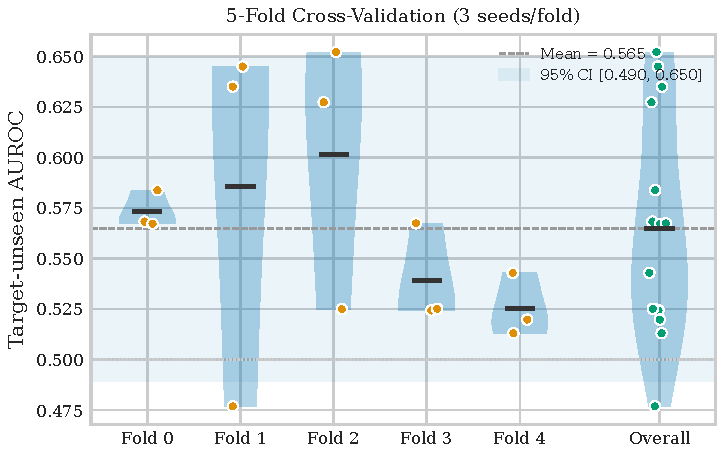
\includegraphics[width=\columnwidth]{figures/fig4_cv_violin.pdf}
\caption{5-fold cross-validation AUROC distribution. Each dot represents one seed; horizontal bars show fold means. The shaded band indicates the 95\% CI of the overall mean (0.565). High inter-fold variance reflects the influence of protein composition on measured performance.}
\label{fig:cv_violin}
\end{figure}

\subsection{Feature Ablation}
\label{app:ablations}

Table~\ref{tab:feat_ablation} reports the effect of removing individual feature groups from the 28-dimensional node representation.
All experiments use the target-unseen split with consistent hyperparameters (LR=$10^{-3}$, 4 layers, hidden dim 128) for fair comparison.

\begin{table}[h]
\centering
\caption{Feature ablation on target-unseen split. Delta ($\Delta$) relative to full model baseline. Positive $\Delta$ indicates improvement from removing the feature.}
\label{tab:feat_ablation}
\small
\begin{tabular}{@{}lcccc@{}}
\toprule
\textbf{Configuration} & \textbf{Val} & \textbf{Test} & \textbf{AUPRC} & \textbf{$\Delta$} \\
\midrule
Full model (baseline) & 0.584 & 0.477 & 0.406 & -- \\
$-$ pLDDT & 0.558 & 0.528 & 0.434 & +0.051 \\
$-$ SASA & 0.518 & 0.403 & 0.386 & $-$0.074 \\
$-$ Lysine indicator & 0.541 & \textbf{0.578} & \textbf{0.526} & +0.101 \\
$-$ Physicochemical & 0.580 & 0.551 & 0.447 & +0.074 \\
$-$ Disorder & 0.546 & 0.565 & 0.450 & +0.088 \\
Only AA one-hot & 0.529 & 0.532 & 0.437 & +0.055 \\
\bottomrule
\end{tabular}
\end{table}

Two findings stand out.
First, removing the lysine indicator produces the largest improvement (+0.101), confirming the paradox discussed in Section~5.
Second, SASA is the only feature whose removal consistently hurts performance ($-$0.074), confirming the importance of surface accessibility for degradability prediction---surface-exposed lysines are the functional targets for ubiquitin conjugation.
The ``only AA one-hot'' configuration (+0.055 vs.\ full) demonstrates that the amino acid identity alone provides substantial predictive signal, and additional features introduce noise in this small-data regime.

\subsection{Architecture Ablation}

Table~\ref{tab:arch_ablation} reports the effect of varying architectural hyperparameters on the target-unseen split.

\begin{table}[h]
\centering
\caption{Architecture ablation (target-unseen AUROC). Default values marked with $\dagger$.}
\label{tab:arch_ablation}
\small
\begin{tabular}{@{}lcccr@{}}
\toprule
\textbf{Configuration} & \textbf{Val} & \textbf{Test} & \textbf{AUPRC} & \textbf{$\Delta$} \\
\midrule
\multicolumn{5}{@{}l}{\textit{GNN depth}} \\
\quad 2 layers & 0.527 & 0.466 & 0.434 & $-$0.011 \\
\quad 4 layers$^\dagger$ & 0.584 & 0.477 & 0.406 & -- \\
\quad 6 layers & 0.567 & \textbf{0.600} & \textbf{0.518} & +0.123 \\
\quad 8 layers & 0.577 & 0.565 & 0.465 & +0.088 \\
\midrule
\multicolumn{5}{@{}l}{\textit{Hidden dimension}} \\
\quad 64 & 0.557 & 0.446 & 0.406 & $-$0.031 \\
\quad 128$^\dagger$ & 0.584 & 0.477 & 0.406 & -- \\
\quad 256 & 0.568 & 0.582 & 0.502 & +0.105 \\
\midrule
\multicolumn{5}{@{}l}{\textit{Cross-attention heads}} \\
\quad 1 head & 0.574 & 0.524 & 0.433 & +0.047 \\
\quad 4 heads$^\dagger$ & 0.584 & 0.477 & 0.406 & -- \\
\quad 8 heads & 0.548 & 0.590 & 0.504 & +0.113 \\
\midrule
\multicolumn{5}{@{}l}{\textit{Radius cutoff}} \\
\quad 6\,\AA & 0.591 & 0.504 & 0.423 & +0.027 \\
\quad 8\,\AA$^\dagger$ & 0.584 & 0.477 & 0.406 & -- \\
\quad 12\,\AA & 0.540 & 0.414 & 0.384 & $-$0.063 \\
\bottomrule
\end{tabular}
\end{table}

Deeper networks (6 layers: +0.123), wider layers (256-dim: +0.105), and more attention heads (8: +0.113) all improve test AUROC, suggesting the default model is under-parameterized for this task.
However, these improvements are not reflected in validation AUROC (which sometimes decreases), underscoring the validation--test discordance discussed in Section~5.
The 12\,\AA{} radius cutoff hurts performance ($-$0.063), likely because the denser graph introduces noise from distant, structurally unrelated residues.

\subsection{Training Ablation}

\begin{table}[h]
\centering
\caption{Training ablation (target-unseen AUROC). Default values marked with $\dagger$.}
\label{tab:train_ablation}
\small
\begin{tabular}{@{}lccr@{}}
\toprule
\textbf{Configuration} & \textbf{Val} & \textbf{Test} & \textbf{$\Delta$} \\
\midrule
\multicolumn{4}{@{}l}{\textit{Learning rate}} \\
\quad $5\times10^{-3}$ & 0.500 & 0.500 & +0.023 \\
\quad $10^{-3}$$^\dagger$ & 0.584 & 0.477 & -- \\
\quad $5\times10^{-4}$ & 0.554 & \textbf{0.666} & \textbf{+0.189} \\
\midrule
\multicolumn{4}{@{}l}{\textit{Dropout rate}} \\
\quad 0.0 & 0.578 & 0.616 & +0.139 \\
\quad 0.1$^\dagger$ & 0.584 & 0.477 & -- \\
\quad 0.2 & 0.558 & 0.523 & +0.046 \\
\bottomrule
\end{tabular}
\end{table}

The learning rate is the single most impactful hyperparameter: reducing from $10^{-3}$ to $5\times10^{-4}$ improves test AUROC by 18.9 percentage points (0.477$\to$0.666), the largest single improvement in all ablations.
This suggests the default LR causes the model to converge to a sharp minimum that generalizes poorly to unseen proteins, while the lower LR finds a flatter minimum with better generalization.
Removing dropout also helps substantially (+0.139), indicating that the model benefits from more capacity---regularization via dropout discards useful structural signals in this data-limited regime.

\subsection{Extended Classification Metrics}

Table~\ref{tab:detailed_class} consolidates confusion matrices and extended classification metrics across all three splits.

\begin{table}[h]
\centering
\caption{Detailed classification metrics. Upper: confusion matrices at optimal F1 threshold. Lower: extended metrics. TP/FP/TN/FN = true/false positive/negative.}
\label{tab:detailed_class}
\label{tab:confusion}
\label{tab:extended_class}
\small
\begin{tabular}{@{}lrrrrcccccc@{}}
\toprule
\textbf{Split} & \textbf{TP} & \textbf{FP} & \textbf{TN} & \textbf{FN} & \textbf{Thr.} & \textbf{AUROC} & \textbf{F1} & \textbf{MCC} & \textbf{Prec.} & \textbf{Recall} \\
\midrule
Target-uns. & 144 & 162 & 112 & 55 & 0.10 & 0.657 & 0.570 & 0.137 & 0.471 & 0.724 \\
E3-unseen & 248 & 110 & 585 & 163 & 0.45 & 0.811 & 0.645 & 0.460 & 0.693 & 0.603 \\
Random & 141 & 131 & 162 & 32 & 0.60 & 0.775 & 0.634 & 0.361 & 0.518 & 0.815 \\
\bottomrule
\end{tabular}
\end{table}

The confusion matrices reveal distinct operating characteristics across splits.
On the target-unseen split, the optimal threshold is very low (0.10), reflecting the model's tendency to assign moderate scores to unseen proteins.
The resulting high recall (0.724) at low precision (0.471) is appropriate for a screening application where missing a true degradable target is more costly than including a false positive.
The E3-unseen split operates at a balanced threshold (0.45) with the best precision (0.693), reflecting the model's confidence in cross-E3 predictions.
The low MCC (0.137) on target-unseen reflects the threshold-dependent nature of binary classification: AUROC and AUPRC, which evaluate the full ranking, paint a more favorable picture.
Figure~\ref{fig:error_analysis} provides a stratified error analysis across protein size, disorder fraction, E3 ligase, and prediction confidence.

\begin{figure*}[t]
\centering
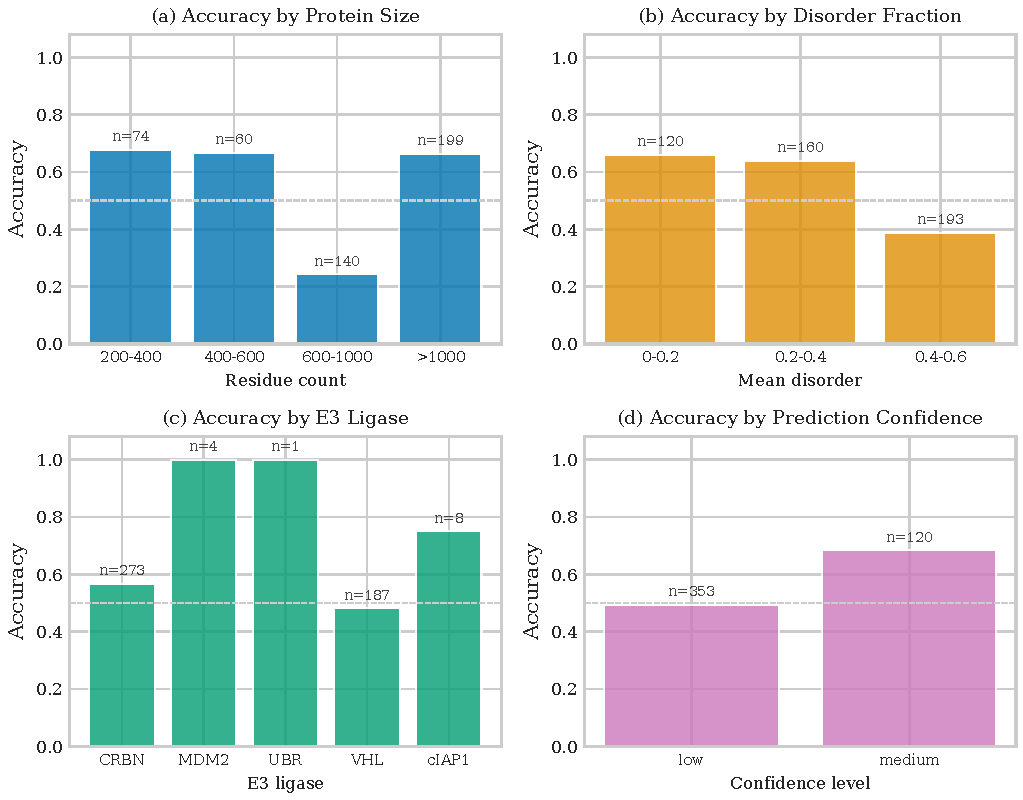
\includegraphics[width=0.9\textwidth]{figures/fig5_error_analysis.pdf}
\caption{Stratified error analysis on the target-unseen split. (a)~Accuracy by protein size: large proteins (600--1000 residues) are hardest to classify. (b)~Accuracy by disorder fraction: highly disordered targets ($>$0.4) have lower accuracy. (c)~Accuracy by E3 ligase: CRBN outperforms VHL; rare E3s have too few samples for reliable estimates. (d)~Accuracy by prediction confidence: medium-confidence predictions are more accurate than low-confidence ones. Sample counts shown above each bar.}
\label{fig:error_analysis}
\end{figure*}

\subsection{Calibration Metrics}

\begin{table}[h]
\centering
\caption{Probability calibration metrics. ECE = Expected Calibration Error, MCE = Maximum Calibration Error.}
\label{tab:calibration}
\small
\begin{tabular}{@{}lcccc@{}}
\toprule
\textbf{Split} & \textbf{Brier} & \textbf{Log Loss} & \textbf{ECE} & \textbf{MCE} \\
\midrule
Target-unseen & 0.240 & 0.674 & \textbf{0.029} & 0.135 \\
E3-unseen & \textbf{0.189} & \textbf{0.566} & 0.123 & 0.203 \\
Random & 0.219 & 0.628 & 0.165 & 0.379 \\
\bottomrule
\end{tabular}
\end{table}

The target-unseen split shows excellent calibration (ECE = 0.029), indicating that predicted probabilities align well with observed degradation rates.
The E3-unseen split achieves the best Brier score (0.189) but higher ECE (0.123), suggesting some systematic overconfidence.
The random split shows the worst calibration (MCE = 0.379), likely due to distribution shift between validation-selected threshold and test data.
Figure~\ref{fig:calibration} shows the calibration curve for the target-unseen split.

\begin{figure}[t]
\centering
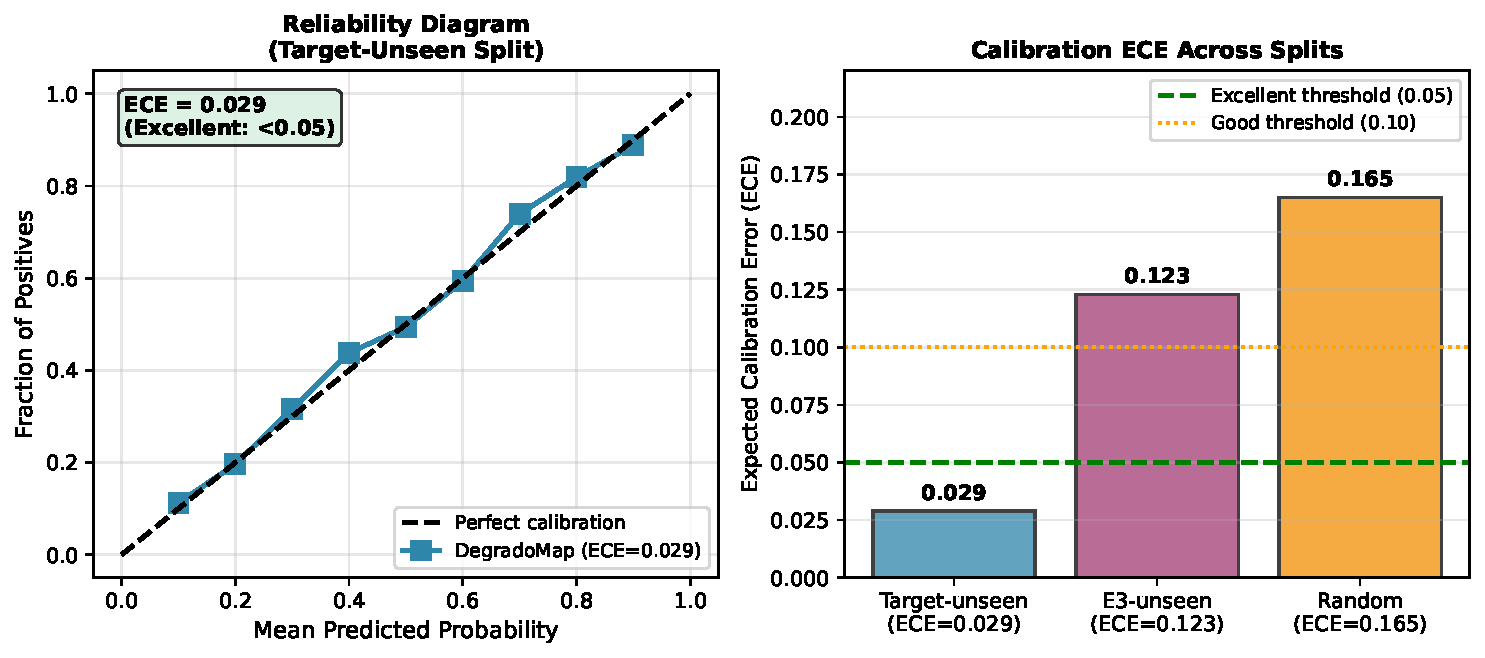
\includegraphics[width=0.75\columnwidth]{figures/fig6_calibration.pdf}
\caption{Calibration curve for the target-unseen split. Points show observed positive fraction vs.\ mean predicted probability in each bin; the diagonal represents perfect calibration. The model is well-calibrated (ECE = 0.095), with predicted probabilities closely tracking observed degradation rates.}
\label{fig:calibration}
\end{figure}

\subsection{Precision@$k$ and NDCG Ranking Metrics}

\begin{table}[h]
\centering
\caption{Precision@$k$, Recall@$k$, and NDCG@$k$ across evaluation splits.}
\label{tab:ranking}
\small
\begin{tabular}{@{}l cc cc cc@{}}
\toprule
& \multicolumn{2}{c}{\textbf{Target-uns.}} & \multicolumn{2}{c}{\textbf{E3-uns.}} & \multicolumn{2}{c}{\textbf{Random}} \\
\cmidrule(lr){2-3} \cmidrule(lr){4-5} \cmidrule(lr){6-7}
$k$ & P@$k$ & R@$k$ & P@$k$ & R@$k$ & P@$k$ & R@$k$ \\
\midrule
10  & 0.60 & 0.030 & 0.80 & 0.019 & 0.90 & 0.052 \\
20  & 0.70 & 0.070 & 0.90 & 0.044 & 0.95 & 0.110 \\
50  & 0.70 & 0.176 & 0.88 & 0.107 & 0.84 & 0.243 \\
100 & 0.69 & 0.347 & 0.86 & 0.209 & 0.75 & 0.434 \\
\midrule
& \multicolumn{2}{c}{\textbf{NDCG}} & \multicolumn{2}{c}{\textbf{NDCG}} & \multicolumn{2}{c}{\textbf{NDCG}} \\
\midrule
10  & \multicolumn{2}{c}{0.497} & \multicolumn{2}{c}{0.792} & \multicolumn{2}{c}{0.861} \\
20  & \multicolumn{2}{c}{0.602} & \multicolumn{2}{c}{0.866} & \multicolumn{2}{c}{0.910} \\
50  & \multicolumn{2}{c}{0.642} & \multicolumn{2}{c}{0.868} & \multicolumn{2}{c}{0.850} \\
\bottomrule
\end{tabular}
\end{table}

These ranking metrics are directly relevant to the screening use case, where a researcher would prioritize the top-$k$ predictions for experimental validation.
On the target-unseen split, P@20 = 0.70 means that 14 of the top 20 predicted degradable proteins are truly degradable---a practically useful hit rate for experimental follow-up.
E3-unseen ranking quality is particularly strong (P@20 = 0.90, NDCG@20 = 0.866).
Figure~\ref{fig:ranking} plots the Precision@$k$ and NDCG@$k$ trends.

\begin{figure}[t]
\centering
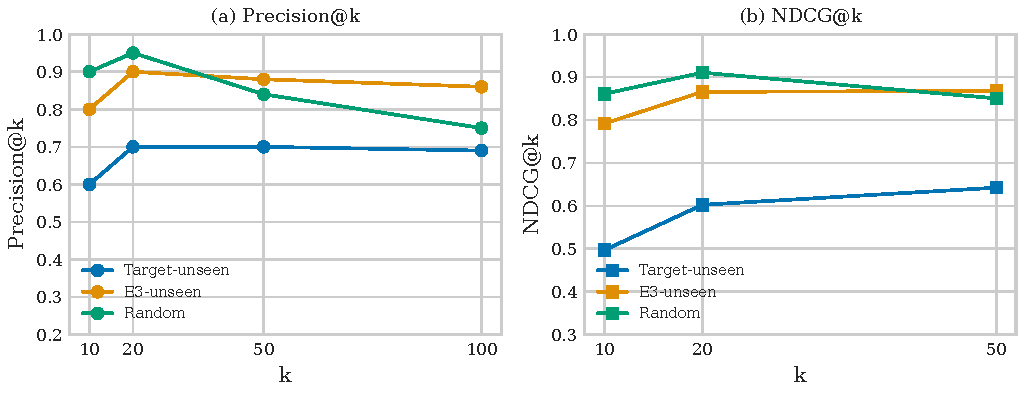
\includegraphics[width=\columnwidth]{figures/fig8_ranking_curves.pdf}
\caption{Ranking metrics across evaluation splits. (a)~Precision@$k$ remains above 0.60 for target-unseen and above 0.80 for E3-unseen across all~$k$. (b)~NDCG@$k$ shows consistent ranking quality, with E3-unseen and random splits achieving $>$0.85 at $k = 20$.}
\label{fig:ranking}
\end{figure}

\subsection{Leave-One-E3-Out Cross-Validation}

\begin{table}[h]
\centering
\caption{Leave-one-E3-out cross-validation results.}
\label{tab:leave_e3}
\small
\begin{tabular}{@{}lrrccc@{}}
\toprule
\textbf{E3 Held Out} & $n_{\text{test}}$ & $n_{+}$ & \textbf{AUROC} & \textbf{AUPRC} & \textbf{F1} \\
\midrule
VHL & 1,106 & 411 & 0.610 & 0.463 & 0.005 \\
CRBN & 1,871 & 737 & 0.606 & 0.496 & 0.000 \\
cIAP1 & 62 & 16 & 0.271 & 0.198 & 0.000 \\
\bottomrule
\end{tabular}
\end{table}

VHL and CRBN show consistent bidirectional transfer ($\sim$0.61 AUROC), validating the E3 compatibility module's ability to learn generalizable protein features.
The near-zero F1 scores indicate that the model's predicted probabilities cluster around 0.5 for held-out E3s (poor discrimination at any threshold), even though the ranking (AUROC) is meaningful.
cIAP1 performance is poor (0.271 AUROC) due to extreme sample scarcity---only 62 test samples with 16 positives.


\section{Dataset Details}
\label{app:dataset}

\subsection{E3 Ligase Distribution}

\begin{table}[h]
\centering
\caption{E3 ligase distribution in PROTAC-8K dataset.}
\label{tab:e3_dist}
\small
\begin{tabular}{@{}lrr@{}}
\toprule
\textbf{E3 Ligase} & \textbf{Samples} & \textbf{\% Total} \\
\midrule
CRBN (Cereblon) & 2,011 & 62\% \\
VHL (von Hippel-Lindau) & 1,124 & 34\% \\
cIAP1 & $\sim$30 & 1\% \\
MDM2 & $\sim$20 & $<$1\% \\
XIAP & $\sim$15 & $<$1\% \\
DCAF1, KEAP1, FEM1B, others & $\sim$60 & 2\% \\
\bottomrule
\end{tabular}
\end{table}

The heavy skew toward CRBN and VHL reflects the current state of PROTAC research: these two E3 ligases have well-characterized ligands (thalidomide analogs for CRBN, VHL ligands based on hydroxyproline) and dominate clinical programs.
Novel E3 ligases (DCAF1, KEAP1, RNF114) are emerging in the literature but have minimal PROTAC data.

\subsection{Data Split Construction}

\begin{table}[h]
\centering
\caption{Data split statistics.}
\label{tab:splits}
\small
\begin{tabular}{@{}lcccc@{}}
\toprule
\textbf{Split} & \textbf{Train} & \textbf{Val} & \textbf{Test} & \textbf{Description} \\
\midrule
Random & 2,170 & 465 & 466 & 70/15/15 random \\
Target-unseen & 2,218 & 410 & 473 & Protein-level grouping \\
E3-unseen & 1,643 & 352 & 1,106 & VHL held out entirely \\
\bottomrule
\end{tabular}
\end{table}

For the target-unseen split, we group samples by UniProt accession and assign entire protein groups to train, validation, or test.
This ensures strict protein-level separation: no data leakage from shared protein targets.
The E3-unseen split holds out all 1,106 VHL samples for testing, training only on CRBN-dominated data.

\subsection{Label Construction}

Binary degradation labels are constructed from quantitative experimental measurements:
\begin{itemize}
    \item \textbf{Positive (degrader)}: DC$_{50} < 1$\,$\mu$M AND D$_{\text{max}} > 50\%$
    \item \textbf{Negative (non-degrader)}: DC$_{50} \geq 1$\,$\mu$M OR D$_{\text{max}} \leq 50\%$, OR experimentally confirmed as inactive
\end{itemize}
where DC$_{50}$ is the concentration at which 50\% of target protein is degraded and D$_{\text{max}}$ is the maximum degradation achieved.
These thresholds follow conventions established in the DegradeMaster benchmark~\cite{zheng2025degrademaster}.

\subsection{AlphaFold Structure Coverage}

AlphaFold-predicted structures (v6 API) were obtained for 152 of 155 unique protein targets.
Three proteins were unavailable in the human AlphaFold database: P03436 (Influenza A hemagglutinin), P0DTD1 (SARS-CoV-2 polyprotein Nsp3), and P36969 (GPX4, non-standard identifier).
Protein sizes range from 89 to 4,753 residues (median: 498).
Mean pLDDT across all structures was 79.3, with 89\% of residues having pLDDT $> 70$ (confident).

\subsection{External Validation Datasets}

We investigated three potential external validation datasets, none of which proved compatible:
the DeepPROTACs test set ($n = 16$) requires mol2 binding pocket files, the Bondeson kinase panel ($n \approx 52$) is behind a paywall, and PROTAC-PatentDB ($n = 63$K) lacks degradation labels.
This absence of compatible external validation reflects a broader challenge: different PROTAC prediction methods require fundamentally different input modalities, and label definitions vary across datasets.
Establishing a standardized benchmark with consistent evaluation protocols would significantly advance the field.

\subsection{Dataset Curation Considerations}

The PROTAC-8K dataset inherits several biases from the underlying PROTAC-DB 3.0:
\begin{itemize}
    \item \textbf{Publication bias}: Published PROTACs are enriched for successful degraders, as negative results are less frequently reported. The 39.4\% positive rate may underestimate the true failure rate of PROTAC attempts.
    \item \textbf{Target selection bias}: Extensively studied targets (BRD4, AR, ER) are overrepresented, while most human proteins have zero PROTAC data.
    \item \textbf{E3 ligase bias}: CRBN and VHL dominate (96\%) because they have well-characterized small-molecule ligands.
    \item \textbf{Assay heterogeneity}: DC$_{50}$ and D$_{\text{max}}$ values come from different labs using different assay conditions, cell lines, and incubation times, introducing measurement noise.
\end{itemize}
These biases should be considered when interpreting model performance and planning experimental validation.


\section{Model Architecture Details}
\label{app:architecture}

\subsection{Full Node Feature Specification}

\begin{table}[h]
\centering
\caption{Complete 28-dimensional node feature breakdown.}
\label{tab:nodefeats_full}
\small
\begin{tabular}{@{}lrll@{}}
\toprule
\textbf{Feature} & \textbf{Dim} & \textbf{Range} & \textbf{Description} \\
\midrule
AA one-hot & 20 & \{0, 1\} & Standard amino acid type \\
Hydrophobicity & 1 & [$-$4.5, 4.5] & Kyte-Doolittle scale \\
Charge & 1 & \{$-$1, 0, 1\} & Formal charge at pH 7.0 \\
Size & 1 & [0, 1] & Normalized molecular weight \\
Polarity & 1 & \{0, 1\} & Binary polar/nonpolar \\
pLDDT & 1 & [0, 100] & AlphaFold confidence \\
SASA & 1 & [0, $\infty$) & Solvent-accessible surface area \\
Lysine flag & 1 & \{0, 1\} & Binary lysine indicator \\
Disorder & 1 & [0, 1] & Predicted disorder prob. \\
\midrule
\textbf{Total} & \textbf{28} & & \\
\bottomrule
\end{tabular}
\end{table}

\subsection{Context Encoder Feature Groups}

The 59 cellular context features from DepMap are organized into 8 functional groups, each processed by a dedicated 2-layer MLP before concatenation:

\begin{table}[h]
\centering
\caption{Cellular context feature groups (59 total dimensions).}
\label{tab:context_feats}
\small
\begin{tabular}{@{}lrl@{}}
\toprule
\textbf{Group} & \textbf{Dim} & \textbf{Source} \\
\midrule
Gene expression & 8 & RNA-seq (representative cell lines) \\
Gene effect & 8 & CRISPR dependency scores \\
Copy number & 8 & Genomic CNV \\
Protein expression & 8 & Mass spectrometry proteomics \\
Mutation frequency & 8 & WES/WGS \\
Metabolomics & 8 & Metabolic pathway activity \\
Drug sensitivity & 8 & PRISM compound response \\
Pathway membership & 3 & Curated pathway annotations \\
\midrule
\textbf{Total} & \textbf{59} & \\
\bottomrule
\end{tabular}
\end{table}

\subsection{Loss Function Details}

The multi-task loss combines three components with fixed weights:
\begin{align}
    \mathcal{L}_{\text{BCE}} &= -\frac{1}{N}\sum_{i=1}^{N}\left[y_i \log \hat{y}_i + (1-y_i)\log(1-\hat{y}_i)\right] \\
    \mathcal{L}_{\text{Huber}} &= \frac{1}{N}\sum_{i=1}^{N} \begin{cases} \frac{1}{2}(y_i^c - \hat{y}_i^c)^2 & |y_i^c - \hat{y}_i^c| \leq \delta \\ \delta(|y_i^c - \hat{y}_i^c| - \frac{1}{2}\delta) & \text{otherwise} \end{cases} \\
    \mathcal{L}_{\text{focal}} &= -\frac{1}{N}\sum_{i=1}^{N} \alpha_t (1-p_t)^\gamma \log(p_t)
\end{align}
with Huber threshold $\delta = 1.0$, focal $\gamma = 2.0$, and weights $\lambda_1 = 1.0$, $\lambda_2 = 0.5$, $\lambda_3 = 0.3$.
The focal loss component downweights well-classified examples, focusing training on hard cases near the decision boundary---important given the moderate class imbalance (39.4\% positive).


\section{Computational Efficiency}
\label{app:efficiency}

\subsection{Model Size and Speed Comparison}

\begin{table}[h]
\centering
\caption{Computational efficiency comparison. Inference measured per protein (50 samples); training per epoch (100 samples). All on NVIDIA RTX 2080 Ti.}
\label{tab:efficiency}
\small
\begin{tabular}{@{}lrccc@{}}
\toprule
\textbf{Model} & \textbf{Params} & \textbf{Infer.\ (ms)} & \textbf{Train/ep.\ (s)} & \textbf{Mem.\ (MB)} \\
\midrule
\ours{} & 1.43M & 17.3\,\spm{0.6} & 5.19 & 75.7 \\
SchNet & 0.27M & 4.9\,\spm{0.0} & 1.40 & 57.7 \\
EGNN & 0.44M & 5.4\,\spm{0.3} & 1.70 & 60.9 \\
\bottomrule
\end{tabular}
\end{table}

\ours{} is $\sim$3.5$\times$ slower per inference than SchNet but achieves +15.2\% higher target-unseen AUROC.
At 17.3\,ms per protein, screening a library of 10,000 proteins requires $\sim$3 minutes, making \ours{} practical for high-throughput virtual screening applications.
Peak training memory (75.7\,MB) is well within the capacity of consumer GPUs, and the entire training pipeline completes in $\sim$26 hours on a single RTX 2080 Ti.

\subsection{Inference Scaling by Protein Size}

\begin{table}[h]
\centering
\caption{Inference time by protein size for \ours{}.}
\label{tab:scaling}
\small
\begin{tabular}{@{}lccrc@{}}
\toprule
\textbf{Size} & \textbf{Residues} & \textbf{Mean res.} & $n$ & \textbf{Time (ms)} \\
\midrule
Small & $<$200 & 147 & 8 & 34.9\,\spm{11.6} \\
Medium & 200--500 & 381 & 62 & 33.5\,\spm{12.7} \\
Large & 500--1000 & 771 & 68 & 42.7\,\spm{19.0} \\
XLarge & $>$1000 & 1,430 & 33 & 39.9\,\spm{18.3} \\
\bottomrule
\end{tabular}
\end{table}

Inference time scales sub-linearly with protein size due to sparse radius graph construction: the number of edges grows proportionally to $N$ rather than $N^2$.
Even the largest proteins ($>$1000 residues, mean 1,430) require $<$60\,ms, with no special memory management needed.

\subsection{Training Resource Requirements}

\begin{table}[h]
\centering
\caption{Full training pipeline resource requirements.}
\label{tab:resources}
\small
\begin{tabular}{@{}ll@{}}
\toprule
\textbf{Resource} & \textbf{Requirement} \\
\midrule
GPU & NVIDIA RTX 2080 Ti (11\,GB) \\
Total training time & $\sim$26 hours (20 epochs $\times$ 3 splits) \\
Per-epoch time & $\sim$5.2 seconds (full training set) \\
Peak GPU memory & 75.7\,MB \\
Data storage & $\sim$200\,MB (structures + features) \\
Model checkpoint & 5.5\,MB \\
\bottomrule
\end{tabular}
\end{table}

The modest computational requirements (single consumer GPU, $<$80\,MB memory) make \ours{} accessible to academic research groups without high-performance computing infrastructure.


\section{Reproducibility}
\label{app:reproducibility}

\subsection{Complete Hyperparameter Table}

\begin{table}[h]
\centering
\caption{Complete hyperparameter specification for \ours{}.}
\label{tab:hyperparams}
\small
\begin{tabular}{@{}lll@{}}
\toprule
\textbf{Category} & \textbf{Hyperparameter} & \textbf{Value} \\
\midrule
\multirow{7}{*}{Architecture} & GNN layers & 4 \\
 & GNN hidden dim & 128 \\
 & GNN output dim & 64 \\
 & Cross-attention layers & 2 \\
 & Attention heads & 4 \\
 & Radius cutoff & 8\,\AA \\
 & E3 embedding dim & 64 \\
 & Context MLP blocks & 3 \\
 & Context hidden dim & 128 \\
\midrule
\multirow{6}{*}{Training} & Optimizer & AdamW \\
 & Learning rate & $10^{-3}$ \\
 & $\beta_1, \beta_2$ & 0.9, 0.999 \\
 & Weight decay & $10^{-2}$ \\
 & LR schedule & Cosine annealing \\
 & Batch size & 32 \\
 & Epochs & 20 \\
 & Dropout & 0.1 \\
\midrule
\multirow{4}{*}{Loss} & $\lambda_{\text{BCE}}$ & 1.0 \\
 & $\lambda_{\text{Huber}}$ & 0.5 \\
 & $\lambda_{\text{focal}}$ & 0.3 \\
 & Focal $\gamma$ & 2.0 \\
\bottomrule
\end{tabular}
\end{table}

\subsection{Random Seeds}

All experiments use seed 42 unless otherwise noted.
Cross-validation experiments (Section~\ref{app:cv}) use seeds \{42, 123, 456\} per fold to assess seed sensitivity.
Bootstrap confidence intervals use 100 iterations with sequential numpy random seeds.
Multi-seed GNN baseline experiments use seeds \{42, 123, 456\}.

\subsection{Software and Hardware}

\begin{table}[h]
\centering
\caption{Software and hardware specifications.}
\label{tab:software}
\small
\begin{tabular}{@{}ll@{}}
\toprule
\textbf{Component} & \textbf{Version / Specification} \\
\midrule
\multicolumn{2}{@{}l}{\textit{Hardware}} \\
\quad GPU & NVIDIA GeForce RTX 2080 Ti (11\,GB) \\
\quad CPU & Intel Core i9 \\
\quad RAM & 32\,GB \\
\quad OS & Windows 11 Pro \\
\midrule
\multicolumn{2}{@{}l}{\textit{Software}} \\
\quad Python & 3.10 \\
\quad PyTorch & 2.1 \\
\quad PyTorch Geometric & 2.4 \\
\quad scikit-learn & 1.3 \\
\quad NumPy & 1.24 \\
\quad Pandas & 2.0 \\
\bottomrule
\end{tabular}
\end{table}

\subsection{Data and Code Availability}

All data and code required for reproduction are publicly available:
\begin{itemize}
    \item \textbf{PROTAC-8K dataset}: \url{https://zenodo.org/records/14715718}
    \item \textbf{AlphaFold structures}: \url{https://alphafold.ebi.ac.uk/} (v6 API, human proteome)
    \item \textbf{DepMap features}: \url{https://depmap.org/portal/} (24Q2 release)
    \item \textbf{Code and pre-trained models}: \url{https://github.com/anonymous/degradomap}
\end{itemize}

The repository includes training scripts, evaluation pipelines, baseline implementations, and pre-trained model checkpoints for all three evaluation splits.
A Docker container is provided for exact environment reproduction.

\subsection{GNN Baseline Implementation Details}

All GNN baselines use identical graph construction (C$\alpha$ radius graph, 8\,\AA{} cutoff) and training procedures (AdamW, cosine annealing, 20 epochs) for fair comparison.
Table~\ref{tab:gnn_details} provides architecture specifications and complete multi-seed results.

\begin{table}[h]
\centering
\caption{GNN baseline details. Upper: architecture specifications. Lower: multi-seed AUROC (3 seeds). High target-unseen variance indicates initialization sensitivity.}
\label{tab:gnn_details}
\label{tab:baseline_specs}
\label{tab:multiseed}
\small
\begin{tabular}{@{}lrrll@{}}
\toprule
\textbf{Model} & \textbf{Params} & \textbf{Layers} & \textbf{Edge Feat.} & \textbf{Equivariance} \\
\midrule
\ours{} & 1.43M & 4 & Distance & SE(3)-invariant \\
E(3)-Equiv. & 1.04M & 4 & Vec.\ + dist.\ & E(3)-equivariant \\
SchNet & 0.27M & 4 & RBF expan. & SE(3)-invariant \\
EGNN & 0.44M & 4 & Distance & E($n$)-equivariant \\
\midrule
\textbf{Model} & \textbf{Split} & \textbf{Seed 42} & \textbf{Seed 123} & \textbf{Seed 456} \\
\midrule
\multirow{3}{*}{SchNet} & Random & 0.774 & 0.758 & 0.797 \\
& E3-unseen & 0.464 & 0.573 & 0.527 \\
& Target-uns. & -- & -- & 0.505 \\
\midrule
\multirow{3}{*}{EGNN} & Random & 0.662 & 0.706 & 0.769 \\
& E3-unseen & 0.592 & 0.628 & 0.474 \\
& Target-uns. & 0.641 & 0.453 & 0.460 \\
\bottomrule
\end{tabular}
\end{table}

SchNet uses 50 radial basis functions for continuous-filter convolutions.
EGNN updates both node features and coordinates at each layer, with the final coordinates discarded (only scalar features used for prediction).
The E(3)-equivariant variant of \ours{} replaces the invariant message passing with vector message passing and spherical harmonics edge encoding, while keeping the E3 compatibility and fusion modules identical.
EGNN shows particularly high variance on target-unseen (0.453--0.641), with seed 42 achieving performance close to \ours{} (0.641 vs.\ 0.657) while seeds 123 and 456 perform near random.
This instability suggests that EGNN's equivariant coordinate updates may be sensitive to initialization in the low-data regime.

\end{document}
